% Options for packages loaded elsewhere
\PassOptionsToPackage{unicode}{hyperref}
\PassOptionsToPackage{hyphens}{url}
\PassOptionsToPackage{dvipsnames,svgnames,x11names}{xcolor}
%
\documentclass[
  number,
  review]{elsarticle}

\usepackage{amsmath,amssymb}
\usepackage{iftex}
\ifPDFTeX
  \usepackage[T1]{fontenc}
  \usepackage[utf8]{inputenc}
  \usepackage{textcomp} % provide euro and other symbols
\else % if luatex or xetex
  \usepackage{unicode-math}
  \defaultfontfeatures{Scale=MatchLowercase}
  \defaultfontfeatures[\rmfamily]{Ligatures=TeX,Scale=1}
\fi
\usepackage{lmodern}
\ifPDFTeX\else  
    % xetex/luatex font selection
\fi
% Use upquote if available, for straight quotes in verbatim environments
\IfFileExists{upquote.sty}{\usepackage{upquote}}{}
\IfFileExists{microtype.sty}{% use microtype if available
  \usepackage[]{microtype}
  \UseMicrotypeSet[protrusion]{basicmath} % disable protrusion for tt fonts
}{}
\makeatletter
\@ifundefined{KOMAClassName}{% if non-KOMA class
  \IfFileExists{parskip.sty}{%
    \usepackage{parskip}
  }{% else
    \setlength{\parindent}{0pt}
    \setlength{\parskip}{6pt plus 2pt minus 1pt}}
}{% if KOMA class
  \KOMAoptions{parskip=half}}
\makeatother
\usepackage{xcolor}
\setlength{\emergencystretch}{3em} % prevent overfull lines
\setcounter{secnumdepth}{5}
% Make \paragraph and \subparagraph free-standing
\makeatletter
\ifx\paragraph\undefined\else
  \let\oldparagraph\paragraph
  \renewcommand{\paragraph}{
    \@ifstar
      \xxxParagraphStar
      \xxxParagraphNoStar
  }
  \newcommand{\xxxParagraphStar}[1]{\oldparagraph*{#1}\mbox{}}
  \newcommand{\xxxParagraphNoStar}[1]{\oldparagraph{#1}\mbox{}}
\fi
\ifx\subparagraph\undefined\else
  \let\oldsubparagraph\subparagraph
  \renewcommand{\subparagraph}{
    \@ifstar
      \xxxSubParagraphStar
      \xxxSubParagraphNoStar
  }
  \newcommand{\xxxSubParagraphStar}[1]{\oldsubparagraph*{#1}\mbox{}}
  \newcommand{\xxxSubParagraphNoStar}[1]{\oldsubparagraph{#1}\mbox{}}
\fi
\makeatother


\providecommand{\tightlist}{%
  \setlength{\itemsep}{0pt}\setlength{\parskip}{0pt}}\usepackage{longtable,booktabs,array}
\usepackage{calc} % for calculating minipage widths
% Correct order of tables after \paragraph or \subparagraph
\usepackage{etoolbox}
\makeatletter
\patchcmd\longtable{\par}{\if@noskipsec\mbox{}\fi\par}{}{}
\makeatother
% Allow footnotes in longtable head/foot
\IfFileExists{footnotehyper.sty}{\usepackage{footnotehyper}}{\usepackage{footnote}}
\makesavenoteenv{longtable}
\usepackage{graphicx}
\makeatletter
\newsavebox\pandoc@box
\newcommand*\pandocbounded[1]{% scales image to fit in text height/width
  \sbox\pandoc@box{#1}%
  \Gscale@div\@tempa{\textheight}{\dimexpr\ht\pandoc@box+\dp\pandoc@box\relax}%
  \Gscale@div\@tempb{\linewidth}{\wd\pandoc@box}%
  \ifdim\@tempb\p@<\@tempa\p@\let\@tempa\@tempb\fi% select the smaller of both
  \ifdim\@tempa\p@<\p@\scalebox{\@tempa}{\usebox\pandoc@box}%
  \else\usebox{\pandoc@box}%
  \fi%
}
% Set default figure placement to htbp
\def\fps@figure{htbp}
\makeatother

\usepackage{fontspec}
\usepackage{multirow}
\usepackage{multicol}
\usepackage{colortbl}
\usepackage{hhline}
\newlength\Oldarrayrulewidth
\newlength\Oldtabcolsep
\usepackage{longtable}
\usepackage{array}
\usepackage{hyperref}
\usepackage{float}
\usepackage{wrapfig}
\usepackage{longtable}
\usepackage{amsmath}
\usepackage{amssymb}
\usepackage{multicol}
\usepackage{float}
\usepackage{typearea}
\floatplacement{figure}{htbp}
\floatplacement{table}{htbp}
\AtBeginDocument{%
  \storeareas\normalpapersize
}
\BeforeRestoreareas{\cleardoublepage}
\newcommand*\uselandscape{%
  \cleardoublepage
  \KOMAoptions{paper=landscape}%
  \recalctypearea
  \areaset{1.2\textwidth}{1.2\textheight}%
}
\makeatletter
\@ifpackageloaded{caption}{}{\usepackage{caption}}
\AtBeginDocument{%
\ifdefined\contentsname
  \renewcommand*\contentsname{Table of contents}
\else
  \newcommand\contentsname{Table of contents}
\fi
\ifdefined\listfigurename
  \renewcommand*\listfigurename{List of Figures}
\else
  \newcommand\listfigurename{List of Figures}
\fi
\ifdefined\listtablename
  \renewcommand*\listtablename{List of Tables}
\else
  \newcommand\listtablename{List of Tables}
\fi
\ifdefined\figurename
  \renewcommand*\figurename{Figure}
\else
  \newcommand\figurename{Figure}
\fi
\ifdefined\tablename
  \renewcommand*\tablename{Table}
\else
  \newcommand\tablename{Table}
\fi
}
\@ifpackageloaded{float}{}{\usepackage{float}}
\floatstyle{ruled}
\@ifundefined{c@chapter}{\newfloat{codelisting}{h}{lop}}{\newfloat{codelisting}{h}{lop}[chapter]}
\floatname{codelisting}{Listing}
\newcommand*\listoflistings{\listof{codelisting}{List of Listings}}
\makeatother
\makeatletter
\makeatother
\makeatletter
\@ifpackageloaded{caption}{}{\usepackage{caption}}
\@ifpackageloaded{subcaption}{}{\usepackage{subcaption}}
\makeatother
\journal{International Journal of Epidemiology}

\usepackage[]{natbib}
\bibliographystyle{elsarticle-num-names}
\usepackage{bookmark}

\IfFileExists{xurl.sty}{\usepackage{xurl}}{} % add URL line breaks if available
\urlstyle{same} % disable monospaced font for URLs
\hypersetup{
  pdftitle={A temporal network analysis of drug co-prescription during antidepressants and anxiolytics dispensing in the Netherlands from 2018 to 2022},
  pdfauthor={Aly Lamuri; Spyros Balafas; Eelko Hak; Jens H. Bos; Frederike Jörg; Talitha L. Feenstra},
  pdfkeywords={Graph Theory, Prescription
Registry, Co-prescription, Mental Health, Public Health Monitoring},
  colorlinks=true,
  linkcolor={blue},
  filecolor={Maroon},
  citecolor={Blue},
  urlcolor={Blue},
  pdfcreator={LaTeX via pandoc}}


\setlength{\parindent}{6pt}
\begin{document}

\begin{frontmatter}
\title{A temporal network analysis of drug co-prescription during
antidepressants and anxiolytics dispensing in the Netherlands from 2018
to 2022}
\author[1,2]{Aly Lamuri%
\corref{cor1}%
}
 \ead{a.l.m.lamuri.murdani@rug.nl} 
\author[1]{Spyros Balafas%
%
}

\author[1]{Eelko Hak%
%
}

\author[1]{Jens H. Bos%
%
}

\author[1,3]{Frederike Jörg%
%
}

\author[1]{Talitha L. Feenstra%
%
}


\affiliation[1]{organization={University of
Groningen},city={Groningen},country={Netherlands},countrysep={,},postcodesep={}}
\affiliation[2]{organization={University of
Indonesia},city={Depok},country={Indonesia},countrysep={,},postcodesep={}}
\affiliation[3]{organization={University Medical Centre
Groningen},city={Groningen},country={Netherlands},countrysep={,},postcodesep={}}

\cortext[cor1]{Corresponding author}






        
\begin{abstract}
\textbf{Background:} Drug prescription networks (DPNs) model the
temporal dynamics of medication co-prescription within a population.
Understanding these networks can provide insights into polypharmacy and
prescribing behaviors.

\textbf{Objectives:} This study assesses the structural characteristics
of temporal DPNs derived from daily co-prescriptions of antidepressants,
anxiolytics, and other therapeutic drug classes. By analyzing these
networks using eigenvector centrality, we identify influential
medications and prescribing patterns.

\textbf{Methods:} We utilized the IADB.nl database, including
prescriptions from 128 Dutch pharmacies (2018--2022). A cohort of
patients prescribed antidepressants/anxiolytics was extracted.
Medications were classified using the Anatomical Therapeutic Chemical
(ATC) system into 24 therapeutic classes. Time-varying DPNs were
constructed as undirected graphs using symmetric daily dose-adjusted
co-prescriptions. Eigenvector centrality (\(c_e\)) quantified relative
nodal importance. Weekly-aggregated data included prescriptions
(\(n_c\)), number of patients, claim-to-patient ratio, and eigenvector
centrality. Singular spectrum analysis decomposed trends.

\textbf{Results:} Antidepressants (\(c_e\): 0.09, \(n_c\): 28,993) and
anxiolytics (\(c_e\): 0.05, \(n_c\): 14,061) had high eigenvector
centrality, demonstrating frequent co-prescription. Other ATC groups
with high centrality included those for the alimentary tract and
metabolism (\texttt{A01-A16}), blood and blood-forming organs
(\texttt{B01-B06}), cardiovascular system (\texttt{C01-C10}),
respiratory system (\texttt{R01-R07}), and analgesics (\texttt{N02}).

\textbf{Discussion:} DPNs revealed key co-prescription patterns.
High-centrality medications highlight potential targets for drug
monitoring, such as identifying co-prescription trends that may warrant
evaluation for safety, appropriateness, or policy oversight. This
approach aids in identifying influential medications and refining
prescribing oversight.
\end{abstract}





\begin{keyword}
    Graph Theory \sep Prescription
Registry \sep Co-prescription \sep Mental Health \sep 
    Public Health Monitoring
\end{keyword}
\end{frontmatter}
    

\section{Introduction}\label{introduction}

The complexity of health-related phenomena has led to the growing
application of network analysis in medicine and epidemiology
\citep{Luke2007, Miglio2021}. Graph theory provides the mathematical
foundation for network analysis, offering an approach to study the
relationships among the entities of a complex system. The early
implementations of network analysis focused primarily on transmission,
social, and organizational networks. More recently, \citet{Cavallo2012}
introduced drug prescription networks (DPNs) to model population-level
drug prescription data. \citet{Bazzoni2015} formalized the term,
emphasizing its utility in understanding polypharmacy.

Psychiatric polypharmacy is defined as a patient with at least two
concurrent psychiatric medications \citep{Shrivastava2013}. With a
prevalence between 13-90\%, psychiatric polypharmacy manifests in five
categories, namely same-class, multi-class, adjunctive, augmentation,
and total polypharmacy \citep{Shrivastava2013}. Same-class polypharmacy
is the use of multiple medications from the same class. Multi-class
polypharmacy is the use of multiple medications from different classes
indicated for the same symptom cluster. Adjunctive polypharmacy is the
use of additional medications to treat side effects due to other
medications. Augmentation polypharmacy is the use of full-dose and
sub-dose medications from a different class for the same symptom
cluster. Finally, total polypharmacy is the overall number of
medications a patient uses, including those prescribed for multiple
psychiatric symptom clusters as well as for comorbid non-psychiatric
conditions \citep{Shrivastava2013}. For policymakers, differences in
defining polypharmacy pose a challenge to design an effective monitoring
system \citep{Sirois2016}. Such monitoring is essential to identify
prevalent co-prescription pattern that may impact treatment
appropriateness and healthcare policy development.

A DPN is a graphical representation where medications correspond to
nodes, and edges represent co-prescription relationships between them.
Typically, simple undirected graphs are represented by a square
symmetric adjacency matrix \(A\), where each nonzero element \(A_{ij}\)
indicates that medications \(i\) and \(j\) were co-prescribed on a given
day. A population-level DPN can be constructed by aggregating individual
patient networks through matrix addition \citep{Cavallo2012}. Analyzing
the structural characteristics of a DPN using both local
(medication-level) and global (network-level) graph measures provides
insights into co-prescription dynamics.

A DPN for an individual on a given day can be formalized as a simple
undirected graph where medications correspond to nodes, and edges
connecting pairs of nodes represent co-prescription relationships
between medications \citep{Cavallo2012}. Typically, simple undirected
graphs are represented by a square symmetric matrix with zeros on the
diagonal called the adjacency matrix \citep{estrada2012structure}. In
the adjacency matrix of the individual-level DPN, nonzero off-diagonal
elements correspond to two medications being co-prescribed on a given
day.

A population-level DPN on a given day can be constructed from
individual-level DPNs through matrix addition of the corresponding
adjacency matrices \citep{Cavallo2012}. A DPN at the population level on
a given day is then formulated as a weighted undirected graph, which is
characterized by a weighted adjacency matrix with weights equal to the
counts of medication co-prescription occurrences. Therefore, analyzing
the structural characteristics of a DPN over time using both local
(medication-level) and global (network-level) graph measures offers
valuable insights into co-prescription dynamics and can deepen our
understanding of polypharmacy.

Local network statistics, such as node centrality measures, quantify the
importance of a medication in polypharmacy patterns \citep{Askar2021}.
Addressing concerns about standardized polypharmacy indicators raised by
\citet{Sirois2016} and \citet{Delara2022}, we highlight eigenvector
centrality as a key measure of a medication's connection to highly
prescribed drugs. A high eigenvector centrality suggests frequent
co-prescription with commonly used medications, reflecting prescribing
trends. Building on prior studies \citep{Cavallo2012, Bazzoni2015}, we
hypothesize that eigenvector centrality serves as a meaningful
quantitative indicator of polypharmacy. Therefore, this study aimed to
assess the structural characteristics of temporal DPNs, focusing on the
role of eigenvector centrality in identifying associated medications in
adult patients prescribed for antidepressants or anxiolytics.

\section{Methods}\label{methods}

\subsection{Source of data and study
population}\label{source-of-data-and-study-population}

All data in this study originated from the University of Groningen
IADB.nl, a dynamic pharmacy database containing prescription data since
1994 which still grows expansively. The database covers approximately
128 community pharmacies serving over one million patients and was
accessed on the 20\textsuperscript{th}of September, 2023. All patients
are recorded in the database, irrespective of health care insurance,
where the prescription rates, age, and gender are generalizable to
represent the Netherlands \citep{Visser2013}. The database offers a
longitudinal record, where each individual has a uniquely anonymized
tracking identifier. All records contain fields on the date of
medication dispensing, its quantity, dose regimen, number of days
prescribed, prescribing physicians, and the Anatomical Therapeutic
Chemical (ATC) code. Except for the over the counter drugs and
medication dispensed during hospitalization, all medication records for
each patient are complete, mainly due to high patient-pharmacy
commitment in the Netherlands.

This analysis includes daily medication dispensing from a static cohort
of adults aged 18-65 years old and prescribed for anxiolytics or
antidepressants at least once in the time span from 2018 to 2022.

\subsection{Graph theory}\label{graph-theory}

Mathematically, a simple undirected graph \(\mathcal{G}\) is a pair
\(\mathcal{G} = (\mathcal{V}, \mathcal{E})\), where
\(\mathcal{V} = \left(1, \dots, n \right)\) is the set of nodes and
\(\mathcal{E} = \left(\{i, j\} \ | \ i, j \in \mathcal{V}, \ i \neq j \right)\)
is the finite set of edges with \(\{i, j\} = \{j, i\}\). The adjacency
matrix \(A \in \{0, 1\}^{n \times n}\) of a simple undirected graph
\(\mathcal{G}\) with \(\mathcal{V}\) nodes is a square symmetric matrix
of dimension \(n \times n\) defined as Equation~\ref{eq-graph-theory},
with \(A_{ij} = A_{ji}\) for all \(i, j \in \mathcal{V}\) where
\(i \neq j\). For each day \(t = \left(1, \dots, T \right)\) and each
individual \(p = \left(1, \dots, P \right)\), the adjacency matrix
represented a simple undirected graph \citep{estrada2012structure}.

\begin{equation}\phantomsection\label{eq-graph-theory}{
A_{ij} = 
\begin{cases}
1 & \text{if} \{i, j\} \in \mathcal{E} \\
0 & \text{otherwise}
\end{cases}
}\end{equation}

In a DPN, the node set
\(\mathcal{V} = \{\mathcal{v}_1, \mathcal{v}_2, \dots, \mathcal{v}_n\}\)
represents a finite set of \(n\) medications. Additionally,
\(\mathcal{E}\) is a finite set of edges, where each edge is a pair of
nodes that corresponds to a co-prescription. In an undirected graph, the
order of \(i, j\) does not matter. Typically, undirected graphs do not
contain self connections,
\(\{\mathcal{v}_i, \mathcal{v}_i\} \notin \mathcal{E}\) {[}j{]}.

\subsection{Data pre-processing to build the data
matrix}\label{data-pre-processing-to-build-the-data-matrix}

At the individual level, each patient's daily prescription record at
time \(t\) was encoded into a square matrix \(A_t^{(p)}\), where rows
and columns represent medication classes according to the ATC
classification. An off-diagonal entry \(A_{t_{ij}}^{(p)} = 1\) indicates
that medication classes \(i\) and \(j\) were co-prescribed on the same
day for individual \(p\), while a diagonal entry
\(A_{t_{ii}}^{(p)} = 1\) captures the presence of a single prescription
of medication \(i\). To derive the population-level DPN, all
individual-level daily prescription matrix \(A^{(p)}\) were aggregated
by computing their element-wise sum.

\begin{equation}\phantomsection\label{eq-DPN}{A_t = \displaystyle \sum_i A_t^{(p)}}\end{equation}

The population matrix \(A_t\) captures the frequency of co-prescriptions
(off-diagonal) and single prescriptions (diagonal) across the dataset at
the specified time \(t\). Each element \(A_{t_{ij}}\) in the matrix was
interpreted as the number of patients being prescribed with medication
classes \(i\) and \(j\) on the same day \(t\). \(A_t\) was represented
as a weighted undirected graph, where each node corresponds to a
medication class and edges reflect co-prescription frequencies. In the
original work of DPN, all defined daily dose (DDD) were assumed equal to
1, allowing for applying raw counts as the edge weights. However, since
not all medications have DDD = 1, this assumption could lead to
inaccurate representations. To enhance the accuracy of edge weights, we
introduced a weighting function to adjust the contribution of each
co-prescription. Specifically, each co-prescribed medication class was
assigned a weight \(\omega_j\) based on its DDD value using a Gaussian
kernel centered at the baseline weight \(\omega_B = 1\), i.e., the
expected DDD, with standard deviation \(\sigma = \frac{1}{3}\) to allow
for a gradual reduction in weight as DDD deviates from 1.

\begin{equation}\phantomsection\label{eq-weighted-DDD}{\omega_j = \frac{1}{\frac{\omega_B}{3} \sqrt{2 \pi}} e^{-\frac{1}{2}\left(\frac{DDD - \omega_B}{\omega_B/3}\right)^2}}\end{equation}

The edge weight between medication classes \(i\) and \(j\) was computed
as the average of their individual weights:

\begin{equation}\phantomsection\label{eq-regularize-mtx}{
\stackrel{\textrm{Unregularized}}{
  \begin{bmatrix}
  n_{1, 1} & \dots & n_{1, N} \\
  \vdots & \ddots & \vdots \\
  n_{N, 1} & \dots & n_{N, N} \\
  \end{bmatrix}
}
\quad \to \quad
\stackrel{\textrm{Regularized by } DDD}{
  \begin{bmatrix}
  \frac{1}{2} \cdot \left(\omega_1 + \omega_1 \right) & \dots & \frac{1}{2} \cdot \left(\omega_1 + \omega_N \right) \\
  \vdots & \ddots & \vdots \\
  \frac{1}{2} \cdot \left(\omega_N + \omega_1 \right) & \dots & \frac{1}{2} \cdot \left(\omega_N + \omega_N \right) \\
  \end{bmatrix}
}
}\end{equation}

This weighting approach scaled the edge weight that deviate
substantially from the standard \(\omega_B = 1\), improving
comparability across medication classes. To remain consistent with
standard network representations and avoid confounding self-loops, the
diagonal elements were omitted.

\subsection{Centrality measures in graph
theory}\label{centrality-measures-in-graph-theory}

Centrality measures formalize the identification of important nodes in a
graph \citep{estrada2012structure}. Different node centrality measures
quantify different structural properties of a node. Previous work on
DPNs highlighted four centrality measures that could be used to assess
the importance of a medication within a co-prescription network
\citep{Miglio2021}. Degree centrality in a DPN describes the number of
co-prescription with the medication of interest. High (low) degree
centrality means the medication is often (seldom) co-prescribed.
Betweenness centrality indicates the frequency of a medication
connecting two other medications by the shortest possible path. High
(low) betweenness centrality means the medication is (not) a ``bridge''
between different kind of medications. Closeness centrality is the
average distance between one medication to all other medications in the
DPN. High (low) closeness centrality means that the medication is (not)
commonly co-prescribed. Eigenvector centrality reflects the number of
co-prescription with medications that have vital role in the DPN. High
(low) eigenvector centrality means that the medication is often (seldom)
co-prescribed with other important medications.

The choice of centrality largely depends on the objective of network
analysis. As a general guide, degree centrality is useful to identify
popular medication and monitor drug overuse. Betweenness centrality is
suitable for targeting for drug-interaction study and optimizing therapy
plan. Closeness centrality indicates widely-used key medications and
efficiency in treatment networks. Eigenvector centrality is helpful to
identify influential medications and narrow down high-impact medications
for drug monitoring. We defined high and low eigenvector centrality
relative to the expected value \(\frac{1}{n}\), based on the null model
of uniform connectivity (see ``Determining relative importance''). This
study focused on eigenvector centrality to evaluate which medications
have a significant influence on how antidepressants and anxiolytics are
prescribed. Equation~\ref{eq-eigen-centrality} outlines the calculation
of eigenvector centrality; \(c_i\) and \(c_j\) are the centralities of
node \(\mathcal{v}_i\) and \(\mathcal{v}_j\), respectively; \(\lambda\)
is the eigenvalue; \(A_{ji}\) is an element on row \(j\) and column
\(i\) from an adjacency matrix \(A\), representing the connection
between node \(\mathcal{v}_j\) and \(\mathcal{v}_i\).

\begin{equation}\phantomsection\label{eq-eigen-centrality}{
\displaystyle c_i = \frac{1}{\lambda} \sum_{j \neq i} A_{ji} \cdot c_j
}\end{equation}

\subsection{Data analysis}\label{data-analysis}

\subsubsection{Exploratory descriptive
analysis}\label{exploratory-descriptive-analysis}

The data was extracted as a daily time series and aggregated into weekly
and monthly intervals for analysis. It includes four metrics: daily
prescription dispensing, daily patients, dispensing-to-patient ratio,
and eigenvector centrality. For each metric, a univariate descriptive
analysis was performed, reporting the mean, median, standard deviation,
and interquartile range to summarize centrality and dispersion.

\subsubsection{Exploring seasonality in the
dataset}\label{exploring-seasonality-in-the-dataset}

Exploration on seasonality was done on detrended daily, weekly, and
monthly data by generating seasonal plots and calculating the
autocorrelation (ACF) and partial autocorrelation function (PACF).
Seasonal plots were generated for weekly and yearly pattern by using
daily and monthly data, respectively. To generate the seasonal plots,
the data was first deconstructed based on its period. For daily data,
the weekly period was used; while for monthly data, the yearly period
was used. The weekly period was obtained by creating an ordered value
formatted as year - week, e.g.~\texttt{2018\ -\ W01}. Similarly, monthly
period was obtained by creating an ordered value formatted as year -
month, e.g.~\texttt{2018\ -\ M01}. We then grouped the series by its
deconstructed period and visually examine seasonality as overlapping
pattern in most periods. To substantiate the findings, ACF and PACF
plots were used to check on statistical significance of a given pattern.

\subsubsection{Summarizing
co-prescription}\label{summarizing-co-prescription}

This study explored same-class, multi-class, and total co-prescription
categories. These three groups were selected as they can be directly
inferred from medication dispensing data aggregated at the population
level over the year. The statistics were summarized as prescription-day,
defined as the number of medications dispensed on a given day. For
example, seven medications prescribed for one day account for 7
prescription-days. The mean and standard deviation represented the
average number of prescription-days per person for any co-prescription
regimen.

Although five polypharmacy categories were described by
\citet{Shrivastava2013}, augmentation and adjunctive polypharmacy
require clinical context such as diagnoses to determine the rationale
for combined prescriptions, which is not available in our data source.
Therefore, focusing on the three categories that rely solely on
medication class information is the most reasonable approach for this
study.

\subsubsection{Decomposition with singular spectrum
analysis}\label{decomposition-with-singular-spectrum-analysis}

Classical and seasonal-trend decomposition techniques may not fully
capture complex periodic patterns in time-series data. Singular spectrum
analysis (SSA) is a non-parametric method that leverages Hankel matrix
embedding for decomposition. In this study, SSA was applied to identify
trends and seasonal components in weekly aggregated prescription data.
To better isolate trend and seasonal components, sequential SSA was
applied. First, a basic SSA model with the lag parameter \(L\) = 52 was
used to extract the dominant trend. The residuals were then analyzed
with a second SSA model using \(L = \frac{N}{2}\) to capture complex
periodic patterns. The extracted trend, residuals, and oscillatory
components were evaluated visually and statistically, with Mann-Kendall
trend tests applied to assess long-term changes. A complete
documentation of this approach and its rationale was included in the
supplementary file section S1.1.

\subsubsection{Determining relative
importance}\label{determining-relative-importance}

Since the sum of all eigenvector centralities \(c_i\) in equation
\ref{eq-eigen-centrality} equals 1, the expected eigenvector centrality
for each node in a uniformly connected network is \(\frac{1}{n}\), where
\(n\) is the total number of nodes. In such a network, each node has an
equal probability of being connected to any other, and thus no node is
more ``influential'' than another. This expected value value,
\(\frac{1}{n}\), serves as a baseline under a null model of uniform
connectivity. Assuming eigenvector centrality scores approximately
follow a normal distribution, we applied a one-sample Student's T-test
with Bonferroni correction to assess how much each eigenvector
centrality differs from the expected values. Nodes with \(c_i\) greater
than \(\frac{1}{n}\) were categorized as having high eigenvector
centrality, and those below the expected value were considered low.

\section{Results}\label{results}

\subsection{Description of the
population}\label{description-of-the-population}

IADB recorded 149,071 patients having at least one dispensing of
antidepressants or anxiolytics within five years of data extraction.
Table~\ref{tbl-overview-patient} captures the demographical dynamics of
the population from 2018 to 2022. The ratio of male to female only
varied slightly, and the average age steadily increased over the year.
These findings imply that the population demography stays relatively
stable overtime without any indication of sudden changes.

\global\setlength{\Oldarrayrulewidth}{\arrayrulewidth}

\global\setlength{\Oldtabcolsep}{\tabcolsep}

\setlength{\tabcolsep}{0pt}

\renewcommand*{\arraystretch}{1}



\providecommand{\ascline}[3]{\noalign{\global\arrayrulewidth #1}\arrayrulecolor[HTML]{#2}\cline{#3}}

\begin{longtable}[c]{|p{0.43in}|p{0.94in}|p{0.94in}|p{0.59in}|p{0.85in}|p{0.85in}}

\caption{\label{tbl-overview-patient}Number of participating patients
with at least one dispensing of antidepressants or anxiolytics from 2018
to 2022}

\tabularnewline

\ascline{1.5pt}{666666}{1-6}

\multicolumn{1}{>{\raggedright}m{\dimexpr 0.43in+0\tabcolsep}}{\textcolor[HTML]{000000}{\fontsize{7}{7}\selectfont{\global\setmainfont{DejaVu Sans}{}}}} & \multicolumn{3}{>{\centering}m{\dimexpr 2.47in+4\tabcolsep}}{\textcolor[HTML]{000000}{\fontsize{7}{7}\selectfont{\global\setmainfont{DejaVu Sans}{Number\ of\ Patients\ (\%)}}}} & \multicolumn{2}{>{\centering}m{\dimexpr 1.7in+2\tabcolsep}}{\textcolor[HTML]{000000}{\fontsize{7}{7}\selectfont{\global\setmainfont{DejaVu Sans}{Mean\ Age\ (SD)}}}} \\

\ascline{1.5pt}{666666}{1-6}



\multicolumn{1}{>{\raggedright}m{\dimexpr 0.43in+0\tabcolsep}}{\textcolor[HTML]{000000}{\fontsize{7}{7}\selectfont{\global\setmainfont{DejaVu Sans}{Year}}}} & \multicolumn{1}{>{\centering}m{\dimexpr 0.94in+0\tabcolsep}}{\textcolor[HTML]{000000}{\fontsize{7}{7}\selectfont{\global\setmainfont{DejaVu Sans}{Male}}}} & \multicolumn{1}{>{\centering}m{\dimexpr 0.94in+0\tabcolsep}}{\textcolor[HTML]{000000}{\fontsize{7}{7}\selectfont{\global\setmainfont{DejaVu Sans}{Female}}}} & \multicolumn{1}{>{\centering}m{\dimexpr 0.59in+0\tabcolsep}}{\textcolor[HTML]{000000}{\fontsize{7}{7}\selectfont{\global\setmainfont{DejaVu Sans}{Total}}}} & \multicolumn{1}{>{\centering}m{\dimexpr 0.85in+0\tabcolsep}}{\textcolor[HTML]{000000}{\fontsize{7}{7}\selectfont{\global\setmainfont{DejaVu Sans}{Male}}}} & \multicolumn{1}{>{\centering}m{\dimexpr 0.85in+0\tabcolsep}}{\textcolor[HTML]{000000}{\fontsize{7}{7}\selectfont{\global\setmainfont{DejaVu Sans}{Female}}}} \\

\ascline{1.5pt}{666666}{1-6}\endfirsthead 

\ascline{1.5pt}{666666}{1-6}

\multicolumn{1}{>{\raggedright}m{\dimexpr 0.43in+0\tabcolsep}}{\textcolor[HTML]{000000}{\fontsize{7}{7}\selectfont{\global\setmainfont{DejaVu Sans}{}}}} & \multicolumn{3}{>{\centering}m{\dimexpr 2.47in+4\tabcolsep}}{\textcolor[HTML]{000000}{\fontsize{7}{7}\selectfont{\global\setmainfont{DejaVu Sans}{Number\ of\ Patients\ (\%)}}}} & \multicolumn{2}{>{\centering}m{\dimexpr 1.7in+2\tabcolsep}}{\textcolor[HTML]{000000}{\fontsize{7}{7}\selectfont{\global\setmainfont{DejaVu Sans}{Mean\ Age\ (SD)}}}} \\

\ascline{1.5pt}{666666}{1-6}



\multicolumn{1}{>{\raggedright}m{\dimexpr 0.43in+0\tabcolsep}}{\textcolor[HTML]{000000}{\fontsize{7}{7}\selectfont{\global\setmainfont{DejaVu Sans}{Year}}}} & \multicolumn{1}{>{\centering}m{\dimexpr 0.94in+0\tabcolsep}}{\textcolor[HTML]{000000}{\fontsize{7}{7}\selectfont{\global\setmainfont{DejaVu Sans}{Male}}}} & \multicolumn{1}{>{\centering}m{\dimexpr 0.94in+0\tabcolsep}}{\textcolor[HTML]{000000}{\fontsize{7}{7}\selectfont{\global\setmainfont{DejaVu Sans}{Female}}}} & \multicolumn{1}{>{\centering}m{\dimexpr 0.59in+0\tabcolsep}}{\textcolor[HTML]{000000}{\fontsize{7}{7}\selectfont{\global\setmainfont{DejaVu Sans}{Total}}}} & \multicolumn{1}{>{\centering}m{\dimexpr 0.85in+0\tabcolsep}}{\textcolor[HTML]{000000}{\fontsize{7}{7}\selectfont{\global\setmainfont{DejaVu Sans}{Male}}}} & \multicolumn{1}{>{\centering}m{\dimexpr 0.85in+0\tabcolsep}}{\textcolor[HTML]{000000}{\fontsize{7}{7}\selectfont{\global\setmainfont{DejaVu Sans}{Female}}}} \\

\ascline{1.5pt}{666666}{1-6}\endhead



\multicolumn{1}{>{\raggedright}m{\dimexpr 0.43in+0\tabcolsep}}{\textcolor[HTML]{000000}{\fontsize{7}{7}\selectfont{\global\setmainfont{DejaVu Sans}{2018}}}} & \multicolumn{1}{>{\centering}m{\dimexpr 0.94in+0\tabcolsep}}{\textcolor[HTML]{000000}{\fontsize{7}{7}\selectfont{\global\setmainfont{DejaVu Sans}{42,164\ (36.6\%)}}}} & \multicolumn{1}{>{\centering}m{\dimexpr 0.94in+0\tabcolsep}}{\textcolor[HTML]{000000}{\fontsize{7}{7}\selectfont{\global\setmainfont{DejaVu Sans}{73,124\ (63.4\%)}}}} & \multicolumn{1}{>{\centering}m{\dimexpr 0.59in+0\tabcolsep}}{\textcolor[HTML]{000000}{\fontsize{7}{7}\selectfont{\global\setmainfont{DejaVu Sans}{115,288}}}} & \multicolumn{1}{>{\centering}m{\dimexpr 0.85in+0\tabcolsep}}{\textcolor[HTML]{000000}{\fontsize{7}{7}\selectfont{\global\setmainfont{DejaVu Sans}{48.72\ (12.33)}}}} & \multicolumn{1}{>{\centering}m{\dimexpr 0.85in+0\tabcolsep}}{\textcolor[HTML]{000000}{\fontsize{7}{7}\selectfont{\global\setmainfont{DejaVu Sans}{48.02\ (12.80)}}}} \\





\multicolumn{1}{>{\raggedright}m{\dimexpr 0.43in+0\tabcolsep}}{\textcolor[HTML]{000000}{\fontsize{7}{7}\selectfont{\global\setmainfont{DejaVu Sans}{2019}}}} & \multicolumn{1}{>{\centering}m{\dimexpr 0.94in+0\tabcolsep}}{\textcolor[HTML]{000000}{\fontsize{7}{7}\selectfont{\global\setmainfont{DejaVu Sans}{42,427\ (36.7\%)}}}} & \multicolumn{1}{>{\centering}m{\dimexpr 0.94in+0\tabcolsep}}{\textcolor[HTML]{000000}{\fontsize{7}{7}\selectfont{\global\setmainfont{DejaVu Sans}{73,109\ (63.3\%)}}}} & \multicolumn{1}{>{\centering}m{\dimexpr 0.59in+0\tabcolsep}}{\textcolor[HTML]{000000}{\fontsize{7}{7}\selectfont{\global\setmainfont{DejaVu Sans}{115,536}}}} & \multicolumn{1}{>{\centering}m{\dimexpr 0.85in+0\tabcolsep}}{\textcolor[HTML]{000000}{\fontsize{7}{7}\selectfont{\global\setmainfont{DejaVu Sans}{49.26\ (12.62)}}}} & \multicolumn{1}{>{\centering}m{\dimexpr 0.85in+0\tabcolsep}}{\textcolor[HTML]{000000}{\fontsize{7}{7}\selectfont{\global\setmainfont{DejaVu Sans}{48.54\ (13.02)}}}} \\





\multicolumn{1}{>{\raggedright}m{\dimexpr 0.43in+0\tabcolsep}}{\textcolor[HTML]{000000}{\fontsize{7}{7}\selectfont{\global\setmainfont{DejaVu Sans}{2020}}}} & \multicolumn{1}{>{\centering}m{\dimexpr 0.94in+0\tabcolsep}}{\textcolor[HTML]{000000}{\fontsize{7}{7}\selectfont{\global\setmainfont{DejaVu Sans}{42,010\ (36.6\%)}}}} & \multicolumn{1}{>{\centering}m{\dimexpr 0.94in+0\tabcolsep}}{\textcolor[HTML]{000000}{\fontsize{7}{7}\selectfont{\global\setmainfont{DejaVu Sans}{72,700\ (63.4\%)}}}} & \multicolumn{1}{>{\centering}m{\dimexpr 0.59in+0\tabcolsep}}{\textcolor[HTML]{000000}{\fontsize{7}{7}\selectfont{\global\setmainfont{DejaVu Sans}{114,710}}}} & \multicolumn{1}{>{\centering}m{\dimexpr 0.85in+0\tabcolsep}}{\textcolor[HTML]{000000}{\fontsize{7}{7}\selectfont{\global\setmainfont{DejaVu Sans}{49.77\ (12.79)}}}} & \multicolumn{1}{>{\centering}m{\dimexpr 0.85in+0\tabcolsep}}{\textcolor[HTML]{000000}{\fontsize{7}{7}\selectfont{\global\setmainfont{DejaVu Sans}{49.15\ (13.16)}}}} \\





\multicolumn{1}{>{\raggedright}m{\dimexpr 0.43in+0\tabcolsep}}{\textcolor[HTML]{000000}{\fontsize{7}{7}\selectfont{\global\setmainfont{DejaVu Sans}{2021}}}} & \multicolumn{1}{>{\centering}m{\dimexpr 0.94in+0\tabcolsep}}{\textcolor[HTML]{000000}{\fontsize{7}{7}\selectfont{\global\setmainfont{DejaVu Sans}{42,016\ (36.7\%)}}}} & \multicolumn{1}{>{\centering}m{\dimexpr 0.94in+0\tabcolsep}}{\textcolor[HTML]{000000}{\fontsize{7}{7}\selectfont{\global\setmainfont{DejaVu Sans}{72,532\ (63.3\%)}}}} & \multicolumn{1}{>{\centering}m{\dimexpr 0.59in+0\tabcolsep}}{\textcolor[HTML]{000000}{\fontsize{7}{7}\selectfont{\global\setmainfont{DejaVu Sans}{114,548}}}} & \multicolumn{1}{>{\centering}m{\dimexpr 0.85in+0\tabcolsep}}{\textcolor[HTML]{000000}{\fontsize{7}{7}\selectfont{\global\setmainfont{DejaVu Sans}{50.15\ (13.04)}}}} & \multicolumn{1}{>{\centering}m{\dimexpr 0.85in+0\tabcolsep}}{\textcolor[HTML]{000000}{\fontsize{7}{7}\selectfont{\global\setmainfont{DejaVu Sans}{49.55\ (13.42)}}}} \\





\multicolumn{1}{>{\raggedright}m{\dimexpr 0.43in+0\tabcolsep}}{\textcolor[HTML]{000000}{\fontsize{7}{7}\selectfont{\global\setmainfont{DejaVu Sans}{2022}}}} & \multicolumn{1}{>{\centering}m{\dimexpr 0.94in+0\tabcolsep}}{\textcolor[HTML]{000000}{\fontsize{7}{7}\selectfont{\global\setmainfont{DejaVu Sans}{39,464\ (36.7\%)}}}} & \multicolumn{1}{>{\centering}m{\dimexpr 0.94in+0\tabcolsep}}{\textcolor[HTML]{000000}{\fontsize{7}{7}\selectfont{\global\setmainfont{DejaVu Sans}{67,930\ (63.3\%)}}}} & \multicolumn{1}{>{\centering}m{\dimexpr 0.59in+0\tabcolsep}}{\textcolor[HTML]{000000}{\fontsize{7}{7}\selectfont{\global\setmainfont{DejaVu Sans}{107,394}}}} & \multicolumn{1}{>{\centering}m{\dimexpr 0.85in+0\tabcolsep}}{\textcolor[HTML]{000000}{\fontsize{7}{7}\selectfont{\global\setmainfont{DejaVu Sans}{50.82\ (13.12)}}}} & \multicolumn{1}{>{\centering}m{\dimexpr 0.85in+0\tabcolsep}}{\textcolor[HTML]{000000}{\fontsize{7}{7}\selectfont{\global\setmainfont{DejaVu Sans}{50.38\ (13.50)}}}} \\

\ascline{1.5pt}{666666}{1-6}


\end{longtable}

\arrayrulecolor[HTML]{000000}

\global\setlength{\arrayrulewidth}{\Oldarrayrulewidth}

\global\setlength{\tabcolsep}{\Oldtabcolsep}

\renewcommand*{\arraystretch}{1}

\subsection{Cyclicality and seasonality of medication
dispensing}\label{cyclicality-and-seasonality-of-medication-dispensing}

Visual inspection of daily dispensing volumes revealed consistent weekly
cycles. Dispensing peaked on Monday, with an average of 7,222 {[}SD:
999.79{]} and dropped to its lowest on Saturday, with an average of
2,808 {[}SD: 174.08{]} dispensing. The variation between weekends and
weekdays showed a regular and repeating structure in the data. There was
a large margin of difference between the highest and lowest average
number of prescription dispensed, with a peak on Monday, followed by a
decline throughout the week and the lowest levels occurring during
weekends, as shown in Table~\ref{tbl-overview-daily}. The cyclical
patterns are detailed in the supplementary material section S2.1.
Seasonality was explored as dependencies at daily and weekly lags and
further described in the supplementary material section S2.2.

\global\setlength{\Oldarrayrulewidth}{\arrayrulewidth}

\global\setlength{\Oldtabcolsep}{\tabcolsep}

\setlength{\tabcolsep}{0pt}

\renewcommand*{\arraystretch}{1}



\providecommand{\ascline}[3]{\noalign{\global\arrayrulewidth #1}\arrayrulecolor[HTML]{#2}\cline{#3}}

\begin{longtable}[c]{|p{0.75in}|p{0.91in}|p{0.91in}|p{0.84in}}

\caption{\label{tbl-overview-daily}Daily dispensing from 2018 to 2022
among patients with at least one dispensing of antidepressants or
anxiolytics}

\tabularnewline

\ascline{1.5pt}{666666}{1-4}

\multicolumn{1}{>{\raggedright}m{\dimexpr 0.75in+0\tabcolsep}}{\textcolor[HTML]{000000}{\fontsize{7}{7}\selectfont{\global\setmainfont{DejaVu Sans}{}}}} & \multicolumn{3}{>{\centering}m{\dimexpr 2.66in+4\tabcolsep}}{\textcolor[HTML]{000000}{\fontsize{7}{7}\selectfont{\global\setmainfont{DejaVu Sans}{Number\ of\ Prescriptions\ Dispensed}}}} \\

\ascline{1.5pt}{666666}{1-4}



\multicolumn{1}{>{\raggedright}m{\dimexpr 0.75in+0\tabcolsep}}{\textcolor[HTML]{000000}{\fontsize{7}{7}\selectfont{\global\setmainfont{DejaVu Sans}{Day}}}} & \multicolumn{1}{>{\centering}m{\dimexpr 0.91in+0\tabcolsep}}{\textcolor[HTML]{000000}{\fontsize{7}{7}\selectfont{\global\setmainfont{DejaVu Sans}{Mean\ (SD)}}}} & \multicolumn{1}{>{\centering}m{\dimexpr 0.91in+0\tabcolsep}}{\textcolor[HTML]{000000}{\fontsize{7}{7}\selectfont{\global\setmainfont{DejaVu Sans}{Median\ (IQR)}}}} & \multicolumn{1}{>{\centering}m{\dimexpr 0.84in+0\tabcolsep}}{\textcolor[HTML]{000000}{\fontsize{7}{7}\selectfont{\global\setmainfont{DejaVu Sans}{Range}}}} \\

\ascline{1.5pt}{666666}{1-4}\endfirsthead 

\ascline{1.5pt}{666666}{1-4}

\multicolumn{1}{>{\raggedright}m{\dimexpr 0.75in+0\tabcolsep}}{\textcolor[HTML]{000000}{\fontsize{7}{7}\selectfont{\global\setmainfont{DejaVu Sans}{}}}} & \multicolumn{3}{>{\centering}m{\dimexpr 2.66in+4\tabcolsep}}{\textcolor[HTML]{000000}{\fontsize{7}{7}\selectfont{\global\setmainfont{DejaVu Sans}{Number\ of\ Prescriptions\ Dispensed}}}} \\

\ascline{1.5pt}{666666}{1-4}



\multicolumn{1}{>{\raggedright}m{\dimexpr 0.75in+0\tabcolsep}}{\textcolor[HTML]{000000}{\fontsize{7}{7}\selectfont{\global\setmainfont{DejaVu Sans}{Day}}}} & \multicolumn{1}{>{\centering}m{\dimexpr 0.91in+0\tabcolsep}}{\textcolor[HTML]{000000}{\fontsize{7}{7}\selectfont{\global\setmainfont{DejaVu Sans}{Mean\ (SD)}}}} & \multicolumn{1}{>{\centering}m{\dimexpr 0.91in+0\tabcolsep}}{\textcolor[HTML]{000000}{\fontsize{7}{7}\selectfont{\global\setmainfont{DejaVu Sans}{Median\ (IQR)}}}} & \multicolumn{1}{>{\centering}m{\dimexpr 0.84in+0\tabcolsep}}{\textcolor[HTML]{000000}{\fontsize{7}{7}\selectfont{\global\setmainfont{DejaVu Sans}{Range}}}} \\

\ascline{1.5pt}{666666}{1-4}\endhead



\multicolumn{1}{>{\raggedright}m{\dimexpr 0.75in+0\tabcolsep}}{\textcolor[HTML]{000000}{\fontsize{7}{7}\selectfont{\global\setmainfont{DejaVu Sans}{Monday}}}} & \multicolumn{1}{>{\centering}m{\dimexpr 0.91in+0\tabcolsep}}{\textcolor[HTML]{000000}{\fontsize{7}{7}\selectfont{\global\setmainfont{DejaVu Sans}{7,222\ (999.79)}}}} & \multicolumn{1}{>{\centering}m{\dimexpr 0.91in+0\tabcolsep}}{\textcolor[HTML]{000000}{\fontsize{7}{7}\selectfont{\global\setmainfont{DejaVu Sans}{7,400\ (524.00)}}}} & \multicolumn{1}{>{\centering}m{\dimexpr 0.84in+0\tabcolsep}}{\textcolor[HTML]{000000}{\fontsize{7}{7}\selectfont{\global\setmainfont{DejaVu Sans}{2,935\ -\ 9,194}}}} \\





\multicolumn{1}{>{\raggedright}m{\dimexpr 0.75in+0\tabcolsep}}{\textcolor[HTML]{000000}{\fontsize{7}{7}\selectfont{\global\setmainfont{DejaVu Sans}{Tuesday}}}} & \multicolumn{1}{>{\centering}m{\dimexpr 0.91in+0\tabcolsep}}{\textcolor[HTML]{000000}{\fontsize{7}{7}\selectfont{\global\setmainfont{DejaVu Sans}{6,793\ (640.76)}}}} & \multicolumn{1}{>{\centering}m{\dimexpr 0.91in+0\tabcolsep}}{\textcolor[HTML]{000000}{\fontsize{7}{7}\selectfont{\global\setmainfont{DejaVu Sans}{6,821\ (483.00)}}}} & \multicolumn{1}{>{\centering}m{\dimexpr 0.84in+0\tabcolsep}}{\textcolor[HTML]{000000}{\fontsize{7}{7}\selectfont{\global\setmainfont{DejaVu Sans}{3,164\ -\ 8,620}}}} \\





\multicolumn{1}{>{\raggedright}m{\dimexpr 0.75in+0\tabcolsep}}{\textcolor[HTML]{000000}{\fontsize{7}{7}\selectfont{\global\setmainfont{DejaVu Sans}{Wednesday}}}} & \multicolumn{1}{>{\centering}m{\dimexpr 0.91in+0\tabcolsep}}{\textcolor[HTML]{000000}{\fontsize{7}{7}\selectfont{\global\setmainfont{DejaVu Sans}{6,865\ (601.11)}}}} & \multicolumn{1}{>{\centering}m{\dimexpr 0.91in+0\tabcolsep}}{\textcolor[HTML]{000000}{\fontsize{7}{7}\selectfont{\global\setmainfont{DejaVu Sans}{6,852\ (566.00)}}}} & \multicolumn{1}{>{\centering}m{\dimexpr 0.84in+0\tabcolsep}}{\textcolor[HTML]{000000}{\fontsize{7}{7}\selectfont{\global\setmainfont{DejaVu Sans}{3,915\ -\ 8,503}}}} \\





\multicolumn{1}{>{\raggedright}m{\dimexpr 0.75in+0\tabcolsep}}{\textcolor[HTML]{000000}{\fontsize{7}{7}\selectfont{\global\setmainfont{DejaVu Sans}{Thursday}}}} & \multicolumn{1}{>{\centering}m{\dimexpr 0.91in+0\tabcolsep}}{\textcolor[HTML]{000000}{\fontsize{7}{7}\selectfont{\global\setmainfont{DejaVu Sans}{7,109\ (592.11)}}}} & \multicolumn{1}{>{\centering}m{\dimexpr 0.91in+0\tabcolsep}}{\textcolor[HTML]{000000}{\fontsize{7}{7}\selectfont{\global\setmainfont{DejaVu Sans}{7,136\ (579.00)}}}} & \multicolumn{1}{>{\centering}m{\dimexpr 0.84in+0\tabcolsep}}{\textcolor[HTML]{000000}{\fontsize{7}{7}\selectfont{\global\setmainfont{DejaVu Sans}{4,156\ -\ 8,608}}}} \\





\multicolumn{1}{>{\raggedright}m{\dimexpr 0.75in+0\tabcolsep}}{\textcolor[HTML]{000000}{\fontsize{7}{7}\selectfont{\global\setmainfont{DejaVu Sans}{Friday}}}} & \multicolumn{1}{>{\centering}m{\dimexpr 0.91in+0\tabcolsep}}{\textcolor[HTML]{000000}{\fontsize{7}{7}\selectfont{\global\setmainfont{DejaVu Sans}{6,726\ (535.52)}}}} & \multicolumn{1}{>{\centering}m{\dimexpr 0.91in+0\tabcolsep}}{\textcolor[HTML]{000000}{\fontsize{7}{7}\selectfont{\global\setmainfont{DejaVu Sans}{6,771\ (597.00)}}}} & \multicolumn{1}{>{\centering}m{\dimexpr 0.84in+0\tabcolsep}}{\textcolor[HTML]{000000}{\fontsize{7}{7}\selectfont{\global\setmainfont{DejaVu Sans}{3,589\ -\ 8,712}}}} \\





\multicolumn{1}{>{\raggedright}m{\dimexpr 0.75in+0\tabcolsep}}{\textcolor[HTML]{000000}{\fontsize{7}{7}\selectfont{\global\setmainfont{DejaVu Sans}{Saturday}}}} & \multicolumn{1}{>{\centering}m{\dimexpr 0.91in+0\tabcolsep}}{\textcolor[HTML]{000000}{\fontsize{7}{7}\selectfont{\global\setmainfont{DejaVu Sans}{2,808\ (174.08)}}}} & \multicolumn{1}{>{\centering}m{\dimexpr 0.91in+0\tabcolsep}}{\textcolor[HTML]{000000}{\fontsize{7}{7}\selectfont{\global\setmainfont{DejaVu Sans}{2,803\ (169.00)}}}} & \multicolumn{1}{>{\centering}m{\dimexpr 0.84in+0\tabcolsep}}{\textcolor[HTML]{000000}{\fontsize{7}{7}\selectfont{\global\setmainfont{DejaVu Sans}{2,293\ -\ 4,533}}}} \\





\multicolumn{1}{>{\raggedright}m{\dimexpr 0.75in+0\tabcolsep}}{\textcolor[HTML]{000000}{\fontsize{7}{7}\selectfont{\global\setmainfont{DejaVu Sans}{Sunday}}}} & \multicolumn{1}{>{\centering}m{\dimexpr 0.91in+0\tabcolsep}}{\textcolor[HTML]{000000}{\fontsize{7}{7}\selectfont{\global\setmainfont{DejaVu Sans}{2,991\ (166.44)}}}} & \multicolumn{1}{>{\centering}m{\dimexpr 0.91in+0\tabcolsep}}{\textcolor[HTML]{000000}{\fontsize{7}{7}\selectfont{\global\setmainfont{DejaVu Sans}{3,010\ (161.25)}}}} & \multicolumn{1}{>{\centering}m{\dimexpr 0.84in+0\tabcolsep}}{\textcolor[HTML]{000000}{\fontsize{7}{7}\selectfont{\global\setmainfont{DejaVu Sans}{2,381\ -\ 3,478}}}} \\

\ascline{1.5pt}{666666}{1-4}


\end{longtable}

\arrayrulecolor[HTML]{000000}

\global\setlength{\arrayrulewidth}{\Oldarrayrulewidth}

\global\setlength{\tabcolsep}{\Oldtabcolsep}

\renewcommand*{\arraystretch}{1}

\subsection{Co-prescription in the
population}\label{co-prescription-in-the-population}

Table~\ref{tbl-res-poly} outlines the type of co-prescription in the
population and reports two statistics: the sum and the mean with its
standard deviation. The sum indicates the total prescription-days of
co-prescription within a year, and the mean with its standard deviation
represents the average number of co-prescription days per person. For
example, in 2018, same-class co-prescription of antidepressants occurred
for a total of 73,528 prescription-days across the population, with an
average of 0.06 prescription-days per person, interpreted as:

\begin{quote}
``For every 100 people treated with antidepressants, there were
approximately 6 days in total during which same-class co-prescription
regimens occurred.''
\end{quote}

While these average numbers per person may appear low, they are not
intended to reflect the absolute epidemiological importance of
co-prescriptions. Instead, prescription-days serve as a relative metric
to compare the extent of co-prescription across categories and over
time. For instance, Table~\ref{tbl-res-poly} shows that multi-class
polypharmacy generally exhibits higher prescription-day values than
same-class polypharmacy among individuals prescribed antidepressants.
Therefore, prescription-day counts should be interpreted in the context
of relative prescribing patterns, rather than as a direct indicator of
epidemiological significance.

\global\setlength{\Oldarrayrulewidth}{\arrayrulewidth}

\global\setlength{\Oldtabcolsep}{\tabcolsep}

\setlength{\tabcolsep}{0pt}

\renewcommand*{\arraystretch}{1}



\providecommand{\ascline}[3]{\noalign{\global\arrayrulewidth #1}\arrayrulecolor[HTML]{#2}\cline{#3}}

\begin{longtable}[c]{|p{0.39in}|p{0.71in}|p{0.71in}|p{0.71in}|p{0.71in}|p{0.71in}|p{0.71in}|p{0.71in}}

\caption{\label{tbl-res-poly}Summary statistics of different psychiatric
co-prescription categories}

\tabularnewline

\ascline{1.5pt}{666666}{1-8}

\multicolumn{2}{>{\raggedright}m{\dimexpr 1.1in+2\tabcolsep}}{\textcolor[HTML]{000000}{\fontsize{7}{7}\selectfont{\global\setmainfont{DejaVu Sans}{}}}} & \multicolumn{2}{>{\centering}m{\dimexpr 1.42in+2\tabcolsep}}{\textcolor[HTML]{000000}{\fontsize{7}{7}\selectfont{\global\setmainfont{DejaVu Sans}{Population\ Level}}}\textcolor[HTML]{000000}{\fontsize{7}{7}\selectfont{\global\setmainfont{DejaVu Sans}{\textsuperscript{1}}}}} & \multicolumn{2}{>{\centering}m{\dimexpr 1.42in+2\tabcolsep}}{\textcolor[HTML]{000000}{\fontsize{7}{7}\selectfont{\global\setmainfont{DejaVu Sans}{Per\ Person\ (Mean\ [SD])}}}\textcolor[HTML]{000000}{\fontsize{7}{7}\selectfont{\global\setmainfont{DejaVu Sans}{\textsuperscript{2}}}}} & \multicolumn{2}{>{\centering}m{\dimexpr 1.42in+2\tabcolsep}}{\textcolor[HTML]{000000}{\fontsize{7}{7}\selectfont{\global\setmainfont{DejaVu Sans}{Total\ Co-prescription}}}\textcolor[HTML]{000000}{\fontsize{7}{7}\selectfont{\global\setmainfont{DejaVu Sans}{\textsuperscript{3}}}}} \\

\ascline{1.5pt}{666666}{1-8}



\multicolumn{1}{>{\raggedright}m{\dimexpr 0.39in+0\tabcolsep}}{\textcolor[HTML]{000000}{\fontsize{7}{7}\selectfont{\global\setmainfont{DejaVu Sans}{Year}}}} & \multicolumn{1}{>{\raggedright}m{\dimexpr 0.71in+0\tabcolsep}}{\textcolor[HTML]{000000}{\fontsize{7}{7}\selectfont{\global\setmainfont{DejaVu Sans}{Medication}}}} & \multicolumn{1}{>{\centering}m{\dimexpr 0.71in+0\tabcolsep}}{\textcolor[HTML]{000000}{\fontsize{7}{7}\selectfont{\global\setmainfont{DejaVu Sans}{Same-class}}}} & \multicolumn{1}{>{\centering}m{\dimexpr 0.71in+0\tabcolsep}}{\textcolor[HTML]{000000}{\fontsize{7}{7}\selectfont{\global\setmainfont{DejaVu Sans}{Multi-class}}}} & \multicolumn{1}{>{\centering}m{\dimexpr 0.71in+0\tabcolsep}}{\textcolor[HTML]{000000}{\fontsize{7}{7}\selectfont{\global\setmainfont{DejaVu Sans}{Same-class}}}} & \multicolumn{1}{>{\centering}m{\dimexpr 0.71in+0\tabcolsep}}{\textcolor[HTML]{000000}{\fontsize{7}{7}\selectfont{\global\setmainfont{DejaVu Sans}{Multi-class}}}} & \multicolumn{1}{>{\centering}m{\dimexpr 0.71in+0\tabcolsep}}{\textcolor[HTML]{000000}{\fontsize{7}{7}\selectfont{\global\setmainfont{DejaVu Sans}{N}}}} & \multicolumn{1}{>{\centering}m{\dimexpr 0.71in+0\tabcolsep}}{\textcolor[HTML]{000000}{\fontsize{7}{7}\selectfont{\global\setmainfont{DejaVu Sans}{Mean\ [SD]}}}} \\

\ascline{1.5pt}{666666}{1-8}\endfirsthead 

\ascline{1.5pt}{666666}{1-8}

\multicolumn{2}{>{\raggedright}m{\dimexpr 1.1in+2\tabcolsep}}{\textcolor[HTML]{000000}{\fontsize{7}{7}\selectfont{\global\setmainfont{DejaVu Sans}{}}}} & \multicolumn{2}{>{\centering}m{\dimexpr 1.42in+2\tabcolsep}}{\textcolor[HTML]{000000}{\fontsize{7}{7}\selectfont{\global\setmainfont{DejaVu Sans}{Population\ Level}}}\textcolor[HTML]{000000}{\fontsize{7}{7}\selectfont{\global\setmainfont{DejaVu Sans}{\textsuperscript{1}}}}} & \multicolumn{2}{>{\centering}m{\dimexpr 1.42in+2\tabcolsep}}{\textcolor[HTML]{000000}{\fontsize{7}{7}\selectfont{\global\setmainfont{DejaVu Sans}{Per\ Person\ (Mean\ [SD])}}}\textcolor[HTML]{000000}{\fontsize{7}{7}\selectfont{\global\setmainfont{DejaVu Sans}{\textsuperscript{2}}}}} & \multicolumn{2}{>{\centering}m{\dimexpr 1.42in+2\tabcolsep}}{\textcolor[HTML]{000000}{\fontsize{7}{7}\selectfont{\global\setmainfont{DejaVu Sans}{Total\ Co-prescription}}}\textcolor[HTML]{000000}{\fontsize{7}{7}\selectfont{\global\setmainfont{DejaVu Sans}{\textsuperscript{3}}}}} \\

\ascline{1.5pt}{666666}{1-8}



\multicolumn{1}{>{\raggedright}m{\dimexpr 0.39in+0\tabcolsep}}{\textcolor[HTML]{000000}{\fontsize{7}{7}\selectfont{\global\setmainfont{DejaVu Sans}{Year}}}} & \multicolumn{1}{>{\raggedright}m{\dimexpr 0.71in+0\tabcolsep}}{\textcolor[HTML]{000000}{\fontsize{7}{7}\selectfont{\global\setmainfont{DejaVu Sans}{Medication}}}} & \multicolumn{1}{>{\centering}m{\dimexpr 0.71in+0\tabcolsep}}{\textcolor[HTML]{000000}{\fontsize{7}{7}\selectfont{\global\setmainfont{DejaVu Sans}{Same-class}}}} & \multicolumn{1}{>{\centering}m{\dimexpr 0.71in+0\tabcolsep}}{\textcolor[HTML]{000000}{\fontsize{7}{7}\selectfont{\global\setmainfont{DejaVu Sans}{Multi-class}}}} & \multicolumn{1}{>{\centering}m{\dimexpr 0.71in+0\tabcolsep}}{\textcolor[HTML]{000000}{\fontsize{7}{7}\selectfont{\global\setmainfont{DejaVu Sans}{Same-class}}}} & \multicolumn{1}{>{\centering}m{\dimexpr 0.71in+0\tabcolsep}}{\textcolor[HTML]{000000}{\fontsize{7}{7}\selectfont{\global\setmainfont{DejaVu Sans}{Multi-class}}}} & \multicolumn{1}{>{\centering}m{\dimexpr 0.71in+0\tabcolsep}}{\textcolor[HTML]{000000}{\fontsize{7}{7}\selectfont{\global\setmainfont{DejaVu Sans}{N}}}} & \multicolumn{1}{>{\centering}m{\dimexpr 0.71in+0\tabcolsep}}{\textcolor[HTML]{000000}{\fontsize{7}{7}\selectfont{\global\setmainfont{DejaVu Sans}{Mean\ [SD]}}}} \\

\ascline{1.5pt}{666666}{1-8}\endhead



\multicolumn{1}{>{\raggedright}m{\dimexpr 0.39in+0\tabcolsep}}{\textcolor[HTML]{000000}{\fontsize{7}{7}\selectfont{\global\setmainfont{DejaVu Sans}{2018}}}} & \multicolumn{1}{>{\raggedright}m{\dimexpr 0.71in+0\tabcolsep}}{\textcolor[HTML]{000000}{\fontsize{7}{7}\selectfont{\global\setmainfont{DejaVu Sans}{Antidepressants}}}} & \multicolumn{1}{>{\centering}m{\dimexpr 0.71in+0\tabcolsep}}{\textcolor[HTML]{000000}{\fontsize{7}{7}\selectfont{\global\setmainfont{DejaVu Sans}{73,528}}}} & \multicolumn{1}{>{\centering}m{\dimexpr 0.71in+0\tabcolsep}}{\textcolor[HTML]{000000}{\fontsize{7}{7}\selectfont{\global\setmainfont{DejaVu Sans}{844,789}}}} & \multicolumn{1}{>{\centering}m{\dimexpr 0.71in+0\tabcolsep}}{\textcolor[HTML]{000000}{\fontsize{7}{7}\selectfont{\global\setmainfont{DejaVu Sans}{0.06\ [0.25]}}}} & \multicolumn{1}{>{\centering}m{\dimexpr 0.71in+0\tabcolsep}}{\textcolor[HTML]{000000}{\fontsize{7}{7}\selectfont{\global\setmainfont{DejaVu Sans}{0.69\ [1.17]}}}} & \multicolumn{1}{>{\centering}m{\dimexpr 0.71in+0\tabcolsep}}{\textcolor[HTML]{000000}{\fontsize{7}{7}\selectfont{\global\setmainfont{DejaVu Sans}{7,264,585}}}} & \multicolumn{1}{>{\centering}m{\dimexpr 0.71in+0\tabcolsep}}{\textcolor[HTML]{000000}{\fontsize{7}{7}\selectfont{\global\setmainfont{DejaVu Sans}{5.90\ [4.18]}}}} \\





\multicolumn{1}{>{\raggedright}m{\dimexpr 0.39in+0\tabcolsep}}{\textcolor[HTML]{000000}{\fontsize{7}{7}\selectfont{\global\setmainfont{DejaVu Sans}{2019}}}} & \multicolumn{1}{>{\raggedright}m{\dimexpr 0.71in+0\tabcolsep}}{\textcolor[HTML]{000000}{\fontsize{7}{7}\selectfont{\global\setmainfont{DejaVu Sans}{Antidepressants}}}} & \multicolumn{1}{>{\centering}m{\dimexpr 0.71in+0\tabcolsep}}{\textcolor[HTML]{000000}{\fontsize{7}{7}\selectfont{\global\setmainfont{DejaVu Sans}{75,794}}}} & \multicolumn{1}{>{\centering}m{\dimexpr 0.71in+0\tabcolsep}}{\textcolor[HTML]{000000}{\fontsize{7}{7}\selectfont{\global\setmainfont{DejaVu Sans}{821,726}}}} & \multicolumn{1}{>{\centering}m{\dimexpr 0.71in+0\tabcolsep}}{\textcolor[HTML]{000000}{\fontsize{7}{7}\selectfont{\global\setmainfont{DejaVu Sans}{0.06\ [0.25]}}}} & \multicolumn{1}{>{\centering}m{\dimexpr 0.71in+0\tabcolsep}}{\textcolor[HTML]{000000}{\fontsize{7}{7}\selectfont{\global\setmainfont{DejaVu Sans}{0.65\ [1.13]}}}} & \multicolumn{1}{>{\centering}m{\dimexpr 0.71in+0\tabcolsep}}{\textcolor[HTML]{000000}{\fontsize{7}{7}\selectfont{\global\setmainfont{DejaVu Sans}{7,489,533}}}} & \multicolumn{1}{>{\centering}m{\dimexpr 0.71in+0\tabcolsep}}{\textcolor[HTML]{000000}{\fontsize{7}{7}\selectfont{\global\setmainfont{DejaVu Sans}{5.92\ [4.17]}}}} \\





\multicolumn{1}{>{\raggedright}m{\dimexpr 0.39in+0\tabcolsep}}{\textcolor[HTML]{000000}{\fontsize{7}{7}\selectfont{\global\setmainfont{DejaVu Sans}{2020}}}} & \multicolumn{1}{>{\raggedright}m{\dimexpr 0.71in+0\tabcolsep}}{\textcolor[HTML]{000000}{\fontsize{7}{7}\selectfont{\global\setmainfont{DejaVu Sans}{Antidepressants}}}} & \multicolumn{1}{>{\centering}m{\dimexpr 0.71in+0\tabcolsep}}{\textcolor[HTML]{000000}{\fontsize{7}{7}\selectfont{\global\setmainfont{DejaVu Sans}{74,924}}}} & \multicolumn{1}{>{\centering}m{\dimexpr 0.71in+0\tabcolsep}}{\textcolor[HTML]{000000}{\fontsize{7}{7}\selectfont{\global\setmainfont{DejaVu Sans}{828,043}}}} & \multicolumn{1}{>{\centering}m{\dimexpr 0.71in+0\tabcolsep}}{\textcolor[HTML]{000000}{\fontsize{7}{7}\selectfont{\global\setmainfont{DejaVu Sans}{0.06\ [0.25]}}}} & \multicolumn{1}{>{\centering}m{\dimexpr 0.71in+0\tabcolsep}}{\textcolor[HTML]{000000}{\fontsize{7}{7}\selectfont{\global\setmainfont{DejaVu Sans}{0.65\ [1.13]}}}} & \multicolumn{1}{>{\centering}m{\dimexpr 0.71in+0\tabcolsep}}{\textcolor[HTML]{000000}{\fontsize{7}{7}\selectfont{\global\setmainfont{DejaVu Sans}{7,564,952}}}} & \multicolumn{1}{>{\centering}m{\dimexpr 0.71in+0\tabcolsep}}{\textcolor[HTML]{000000}{\fontsize{7}{7}\selectfont{\global\setmainfont{DejaVu Sans}{5.93\ [4.15]}}}} \\





\multicolumn{1}{>{\raggedright}m{\dimexpr 0.39in+0\tabcolsep}}{\textcolor[HTML]{000000}{\fontsize{7}{7}\selectfont{\global\setmainfont{DejaVu Sans}{2021}}}} & \multicolumn{1}{>{\raggedright}m{\dimexpr 0.71in+0\tabcolsep}}{\textcolor[HTML]{000000}{\fontsize{7}{7}\selectfont{\global\setmainfont{DejaVu Sans}{Antidepressants}}}} & \multicolumn{1}{>{\centering}m{\dimexpr 0.71in+0\tabcolsep}}{\textcolor[HTML]{000000}{\fontsize{7}{7}\selectfont{\global\setmainfont{DejaVu Sans}{75,549}}}} & \multicolumn{1}{>{\centering}m{\dimexpr 0.71in+0\tabcolsep}}{\textcolor[HTML]{000000}{\fontsize{7}{7}\selectfont{\global\setmainfont{DejaVu Sans}{804,264}}}} & \multicolumn{1}{>{\centering}m{\dimexpr 0.71in+0\tabcolsep}}{\textcolor[HTML]{000000}{\fontsize{7}{7}\selectfont{\global\setmainfont{DejaVu Sans}{0.06\ [0.25]}}}} & \multicolumn{1}{>{\centering}m{\dimexpr 0.71in+0\tabcolsep}}{\textcolor[HTML]{000000}{\fontsize{7}{7}\selectfont{\global\setmainfont{DejaVu Sans}{0.64\ [1.12]}}}} & \multicolumn{1}{>{\centering}m{\dimexpr 0.71in+0\tabcolsep}}{\textcolor[HTML]{000000}{\fontsize{7}{7}\selectfont{\global\setmainfont{DejaVu Sans}{7,466,014}}}} & \multicolumn{1}{>{\centering}m{\dimexpr 0.71in+0\tabcolsep}}{\textcolor[HTML]{000000}{\fontsize{7}{7}\selectfont{\global\setmainfont{DejaVu Sans}{5.91\ [4.17]}}}} \\





\multicolumn{1}{>{\raggedright}m{\dimexpr 0.39in+0\tabcolsep}}{\textcolor[HTML]{000000}{\fontsize{7}{7}\selectfont{\global\setmainfont{DejaVu Sans}{2022}}}} & \multicolumn{1}{>{\raggedright}m{\dimexpr 0.71in+0\tabcolsep}}{\textcolor[HTML]{000000}{\fontsize{7}{7}\selectfont{\global\setmainfont{DejaVu Sans}{Antidepressants}}}} & \multicolumn{1}{>{\centering}m{\dimexpr 0.71in+0\tabcolsep}}{\textcolor[HTML]{000000}{\fontsize{7}{7}\selectfont{\global\setmainfont{DejaVu Sans}{74,026}}}} & \multicolumn{1}{>{\centering}m{\dimexpr 0.71in+0\tabcolsep}}{\textcolor[HTML]{000000}{\fontsize{7}{7}\selectfont{\global\setmainfont{DejaVu Sans}{797,843}}}} & \multicolumn{1}{>{\centering}m{\dimexpr 0.71in+0\tabcolsep}}{\textcolor[HTML]{000000}{\fontsize{7}{7}\selectfont{\global\setmainfont{DejaVu Sans}{0.06\ [0.25]}}}} & \multicolumn{1}{>{\centering}m{\dimexpr 0.71in+0\tabcolsep}}{\textcolor[HTML]{000000}{\fontsize{7}{7}\selectfont{\global\setmainfont{DejaVu Sans}{0.64\ [1.12]}}}} & \multicolumn{1}{>{\centering}m{\dimexpr 0.71in+0\tabcolsep}}{\textcolor[HTML]{000000}{\fontsize{7}{7}\selectfont{\global\setmainfont{DejaVu Sans}{7,474,032}}}} & \multicolumn{1}{>{\centering}m{\dimexpr 0.71in+0\tabcolsep}}{\textcolor[HTML]{000000}{\fontsize{7}{7}\selectfont{\global\setmainfont{DejaVu Sans}{5.95\ [4.17]}}}} \\





\multicolumn{1}{>{\raggedright}m{\dimexpr 0.39in+0\tabcolsep}}{\textcolor[HTML]{000000}{\fontsize{7}{7}\selectfont{\global\setmainfont{DejaVu Sans}{2018}}}} & \multicolumn{1}{>{\raggedright}m{\dimexpr 0.71in+0\tabcolsep}}{\textcolor[HTML]{000000}{\fontsize{7}{7}\selectfont{\global\setmainfont{DejaVu Sans}{Anxiolytics}}}} & \multicolumn{1}{>{\centering}m{\dimexpr 0.71in+0\tabcolsep}}{\textcolor[HTML]{000000}{\fontsize{7}{7}\selectfont{\global\setmainfont{DejaVu Sans}{34,122}}}} & \multicolumn{1}{>{\centering}m{\dimexpr 0.71in+0\tabcolsep}}{\textcolor[HTML]{000000}{\fontsize{7}{7}\selectfont{\global\setmainfont{DejaVu Sans}{1,049,590}}}} & \multicolumn{1}{>{\centering}m{\dimexpr 0.71in+0\tabcolsep}}{\textcolor[HTML]{000000}{\fontsize{7}{7}\selectfont{\global\setmainfont{DejaVu Sans}{0.03\ [0.17]}}}} & \multicolumn{1}{>{\centering}m{\dimexpr 0.71in+0\tabcolsep}}{\textcolor[HTML]{000000}{\fontsize{7}{7}\selectfont{\global\setmainfont{DejaVu Sans}{0.85\ [1.21]}}}} & \multicolumn{1}{>{\centering}m{\dimexpr 0.71in+0\tabcolsep}}{\textcolor[HTML]{000000}{\fontsize{7}{7}\selectfont{\global\setmainfont{DejaVu Sans}{7,264,585}}}} & \multicolumn{1}{>{\centering}m{\dimexpr 0.71in+0\tabcolsep}}{\textcolor[HTML]{000000}{\fontsize{7}{7}\selectfont{\global\setmainfont{DejaVu Sans}{5.90\ [4.18]}}}} \\





\multicolumn{1}{>{\raggedright}m{\dimexpr 0.39in+0\tabcolsep}}{\textcolor[HTML]{000000}{\fontsize{7}{7}\selectfont{\global\setmainfont{DejaVu Sans}{2019}}}} & \multicolumn{1}{>{\raggedright}m{\dimexpr 0.71in+0\tabcolsep}}{\textcolor[HTML]{000000}{\fontsize{7}{7}\selectfont{\global\setmainfont{DejaVu Sans}{Anxiolytics}}}} & \multicolumn{1}{>{\centering}m{\dimexpr 0.71in+0\tabcolsep}}{\textcolor[HTML]{000000}{\fontsize{7}{7}\selectfont{\global\setmainfont{DejaVu Sans}{31,955}}}} & \multicolumn{1}{>{\centering}m{\dimexpr 0.71in+0\tabcolsep}}{\textcolor[HTML]{000000}{\fontsize{7}{7}\selectfont{\global\setmainfont{DejaVu Sans}{1,044,683}}}} & \multicolumn{1}{>{\centering}m{\dimexpr 0.71in+0\tabcolsep}}{\textcolor[HTML]{000000}{\fontsize{7}{7}\selectfont{\global\setmainfont{DejaVu Sans}{0.03\ [0.16]}}}} & \multicolumn{1}{>{\centering}m{\dimexpr 0.71in+0\tabcolsep}}{\textcolor[HTML]{000000}{\fontsize{7}{7}\selectfont{\global\setmainfont{DejaVu Sans}{0.83\ [1.18]}}}} & \multicolumn{1}{>{\centering}m{\dimexpr 0.71in+0\tabcolsep}}{\textcolor[HTML]{000000}{\fontsize{7}{7}\selectfont{\global\setmainfont{DejaVu Sans}{7,489,533}}}} & \multicolumn{1}{>{\centering}m{\dimexpr 0.71in+0\tabcolsep}}{\textcolor[HTML]{000000}{\fontsize{7}{7}\selectfont{\global\setmainfont{DejaVu Sans}{5.92\ [4.17]}}}} \\





\multicolumn{1}{>{\raggedright}m{\dimexpr 0.39in+0\tabcolsep}}{\textcolor[HTML]{000000}{\fontsize{7}{7}\selectfont{\global\setmainfont{DejaVu Sans}{2020}}}} & \multicolumn{1}{>{\raggedright}m{\dimexpr 0.71in+0\tabcolsep}}{\textcolor[HTML]{000000}{\fontsize{7}{7}\selectfont{\global\setmainfont{DejaVu Sans}{Anxiolytics}}}} & \multicolumn{1}{>{\centering}m{\dimexpr 0.71in+0\tabcolsep}}{\textcolor[HTML]{000000}{\fontsize{7}{7}\selectfont{\global\setmainfont{DejaVu Sans}{32,249}}}} & \multicolumn{1}{>{\centering}m{\dimexpr 0.71in+0\tabcolsep}}{\textcolor[HTML]{000000}{\fontsize{7}{7}\selectfont{\global\setmainfont{DejaVu Sans}{1,053,849}}}} & \multicolumn{1}{>{\centering}m{\dimexpr 0.71in+0\tabcolsep}}{\textcolor[HTML]{000000}{\fontsize{7}{7}\selectfont{\global\setmainfont{DejaVu Sans}{0.03\ [0.16]}}}} & \multicolumn{1}{>{\centering}m{\dimexpr 0.71in+0\tabcolsep}}{\textcolor[HTML]{000000}{\fontsize{7}{7}\selectfont{\global\setmainfont{DejaVu Sans}{0.83\ [1.17]}}}} & \multicolumn{1}{>{\centering}m{\dimexpr 0.71in+0\tabcolsep}}{\textcolor[HTML]{000000}{\fontsize{7}{7}\selectfont{\global\setmainfont{DejaVu Sans}{7,564,952}}}} & \multicolumn{1}{>{\centering}m{\dimexpr 0.71in+0\tabcolsep}}{\textcolor[HTML]{000000}{\fontsize{7}{7}\selectfont{\global\setmainfont{DejaVu Sans}{5.93\ [4.15]}}}} \\





\multicolumn{1}{>{\raggedright}m{\dimexpr 0.39in+0\tabcolsep}}{\textcolor[HTML]{000000}{\fontsize{7}{7}\selectfont{\global\setmainfont{DejaVu Sans}{2021}}}} & \multicolumn{1}{>{\raggedright}m{\dimexpr 0.71in+0\tabcolsep}}{\textcolor[HTML]{000000}{\fontsize{7}{7}\selectfont{\global\setmainfont{DejaVu Sans}{Anxiolytics}}}} & \multicolumn{1}{>{\centering}m{\dimexpr 0.71in+0\tabcolsep}}{\textcolor[HTML]{000000}{\fontsize{7}{7}\selectfont{\global\setmainfont{DejaVu Sans}{29,912}}}} & \multicolumn{1}{>{\centering}m{\dimexpr 0.71in+0\tabcolsep}}{\textcolor[HTML]{000000}{\fontsize{7}{7}\selectfont{\global\setmainfont{DejaVu Sans}{1,035,388}}}} & \multicolumn{1}{>{\centering}m{\dimexpr 0.71in+0\tabcolsep}}{\textcolor[HTML]{000000}{\fontsize{7}{7}\selectfont{\global\setmainfont{DejaVu Sans}{0.02\ [0.16]}}}} & \multicolumn{1}{>{\centering}m{\dimexpr 0.71in+0\tabcolsep}}{\textcolor[HTML]{000000}{\fontsize{7}{7}\selectfont{\global\setmainfont{DejaVu Sans}{0.82\ [1.16]}}}} & \multicolumn{1}{>{\centering}m{\dimexpr 0.71in+0\tabcolsep}}{\textcolor[HTML]{000000}{\fontsize{7}{7}\selectfont{\global\setmainfont{DejaVu Sans}{7,466,014}}}} & \multicolumn{1}{>{\centering}m{\dimexpr 0.71in+0\tabcolsep}}{\textcolor[HTML]{000000}{\fontsize{7}{7}\selectfont{\global\setmainfont{DejaVu Sans}{5.91\ [4.17]}}}} \\





\multicolumn{1}{>{\raggedright}m{\dimexpr 0.39in+0\tabcolsep}}{\textcolor[HTML]{000000}{\fontsize{7}{7}\selectfont{\global\setmainfont{DejaVu Sans}{2022}}}} & \multicolumn{1}{>{\raggedright}m{\dimexpr 0.71in+0\tabcolsep}}{\textcolor[HTML]{000000}{\fontsize{7}{7}\selectfont{\global\setmainfont{DejaVu Sans}{Anxiolytics}}}} & \multicolumn{1}{>{\centering}m{\dimexpr 0.71in+0\tabcolsep}}{\textcolor[HTML]{000000}{\fontsize{7}{7}\selectfont{\global\setmainfont{DejaVu Sans}{31,527}}}} & \multicolumn{1}{>{\centering}m{\dimexpr 0.71in+0\tabcolsep}}{\textcolor[HTML]{000000}{\fontsize{7}{7}\selectfont{\global\setmainfont{DejaVu Sans}{1,027,019}}}} & \multicolumn{1}{>{\centering}m{\dimexpr 0.71in+0\tabcolsep}}{\textcolor[HTML]{000000}{\fontsize{7}{7}\selectfont{\global\setmainfont{DejaVu Sans}{0.03\ [0.16]}}}} & \multicolumn{1}{>{\centering}m{\dimexpr 0.71in+0\tabcolsep}}{\textcolor[HTML]{000000}{\fontsize{7}{7}\selectfont{\global\setmainfont{DejaVu Sans}{0.82\ [1.16]}}}} & \multicolumn{1}{>{\centering}m{\dimexpr 0.71in+0\tabcolsep}}{\textcolor[HTML]{000000}{\fontsize{7}{7}\selectfont{\global\setmainfont{DejaVu Sans}{7,474,032}}}} & \multicolumn{1}{>{\centering}m{\dimexpr 0.71in+0\tabcolsep}}{\textcolor[HTML]{000000}{\fontsize{7}{7}\selectfont{\global\setmainfont{DejaVu Sans}{5.95\ [4.17]}}}} \\

\ascline{1.5pt}{666666}{1-8}



\multicolumn{8}{>{\raggedright}m{\dimexpr 5.35in+14\tabcolsep}}{\textcolor[HTML]{000000}{\fontsize{7}{7}\selectfont{\global\setmainfont{DejaVu Sans}{\textsuperscript{1}}}}\textcolor[HTML]{000000}{\fontsize{7}{7}\selectfont{\global\setmainfont{DejaVu Sans}{The\ total\ occurrence\ of\ co-prescription\ on\ the\ population\ level/prescription-day.}}}} \\





\multicolumn{8}{>{\raggedright}m{\dimexpr 5.35in+14\tabcolsep}}{\textcolor[HTML]{000000}{\fontsize{7}{7}\selectfont{\global\setmainfont{DejaVu Sans}{\textsuperscript{2}}}}\textcolor[HTML]{000000}{\fontsize{7}{7}\selectfont{\global\setmainfont{DejaVu Sans}{The\ expected\ occurrence\ of\ co-prescription\ per\ person/prescription-day.}}}} \\





\multicolumn{8}{>{\raggedright}m{\dimexpr 5.35in+14\tabcolsep}}{\textcolor[HTML]{000000}{\fontsize{7}{7}\selectfont{\global\setmainfont{DejaVu Sans}{\textsuperscript{3}}}}\textcolor[HTML]{000000}{\fontsize{7}{7}\selectfont{\global\setmainfont{DejaVu Sans}{The\ overall\ number\ of\ medications\ a\ patient\ uses,\ including\ those\ prescribed\ for\ multiple\ psychiatric\ symptom\ clusters\ as\ well\ as\ for\ comorbid\ non-psychiatric\ conditions.}}}} \\





\multicolumn{8}{>{\raggedright}m{\dimexpr 5.35in+14\tabcolsep}}{\textcolor[HTML]{000000}{\fontsize{7}{7}\selectfont{\global\setmainfont{DejaVu Sans}{\textsuperscript{}}}}\textcolor[HTML]{000000}{\fontsize{7}{7}\selectfont{\global\setmainfont{DejaVu Sans}{Prescription\ day\ is\ defined\ as\ the\ number\ of\ dispensed\ medication\ per\ day.}}}} \\





\multicolumn{8}{>{\raggedright}m{\dimexpr 5.35in+14\tabcolsep}}{\textcolor[HTML]{000000}{\fontsize{7}{7}\selectfont{\global\setmainfont{DejaVu Sans}{\textsuperscript{}}}}\textcolor[HTML]{000000}{\fontsize{7}{7}\selectfont{\global\setmainfont{DejaVu Sans}{Multi-class\ co-prescription\ is\ defined\ as\ the\ co-prescription\ of\ medications\ from\ different\ ATC\ classification.}}}} \\




\end{longtable}

\arrayrulecolor[HTML]{000000}

\global\setlength{\arrayrulewidth}{\Oldarrayrulewidth}

\global\setlength{\tabcolsep}{\Oldtabcolsep}

\renewcommand*{\arraystretch}{1}

\subsection{Time-series decomposition}\label{time-series-decomposition}

For brevity, Figure~\ref{fig-ssa} only depicts the decomposition result
of antidepressants dispensed over the years. SSA-based decomposition
separates the trend from its harmonics, as shown in the lower half of
the plot. The trend explains roughly 90\% of the variability, and
harmonics explain 10\%. The first two harmonics, F1 and F2, captured
most of the variability in a series compared to the rest of it. The
trend, F1, and F2 were used to reconstruct the time series. The largest
panel in Figure~\ref{fig-ssa} displays the reconstructed time-series
(green line) overlaid on the original data points (gray line).

Additional decomposition results for other medication classes are
presented in the supplementary section S2.3. Broadly antidepressants
exhibited a steady increasing trend over time, while anxiolytics showed
a gradual decline both in dispensing frequency and eigenvector
centrality. Notably, the decomposition made long-term directional
patterns more discernible across all medication classes, emphasizing the
utility of SSA in isolating interpretable temporal dynamics from complex
dispensing data. These decomposed trends provides the reconstructed data
for the subsequent analysis.

\begin{figure}[H]

\centering{

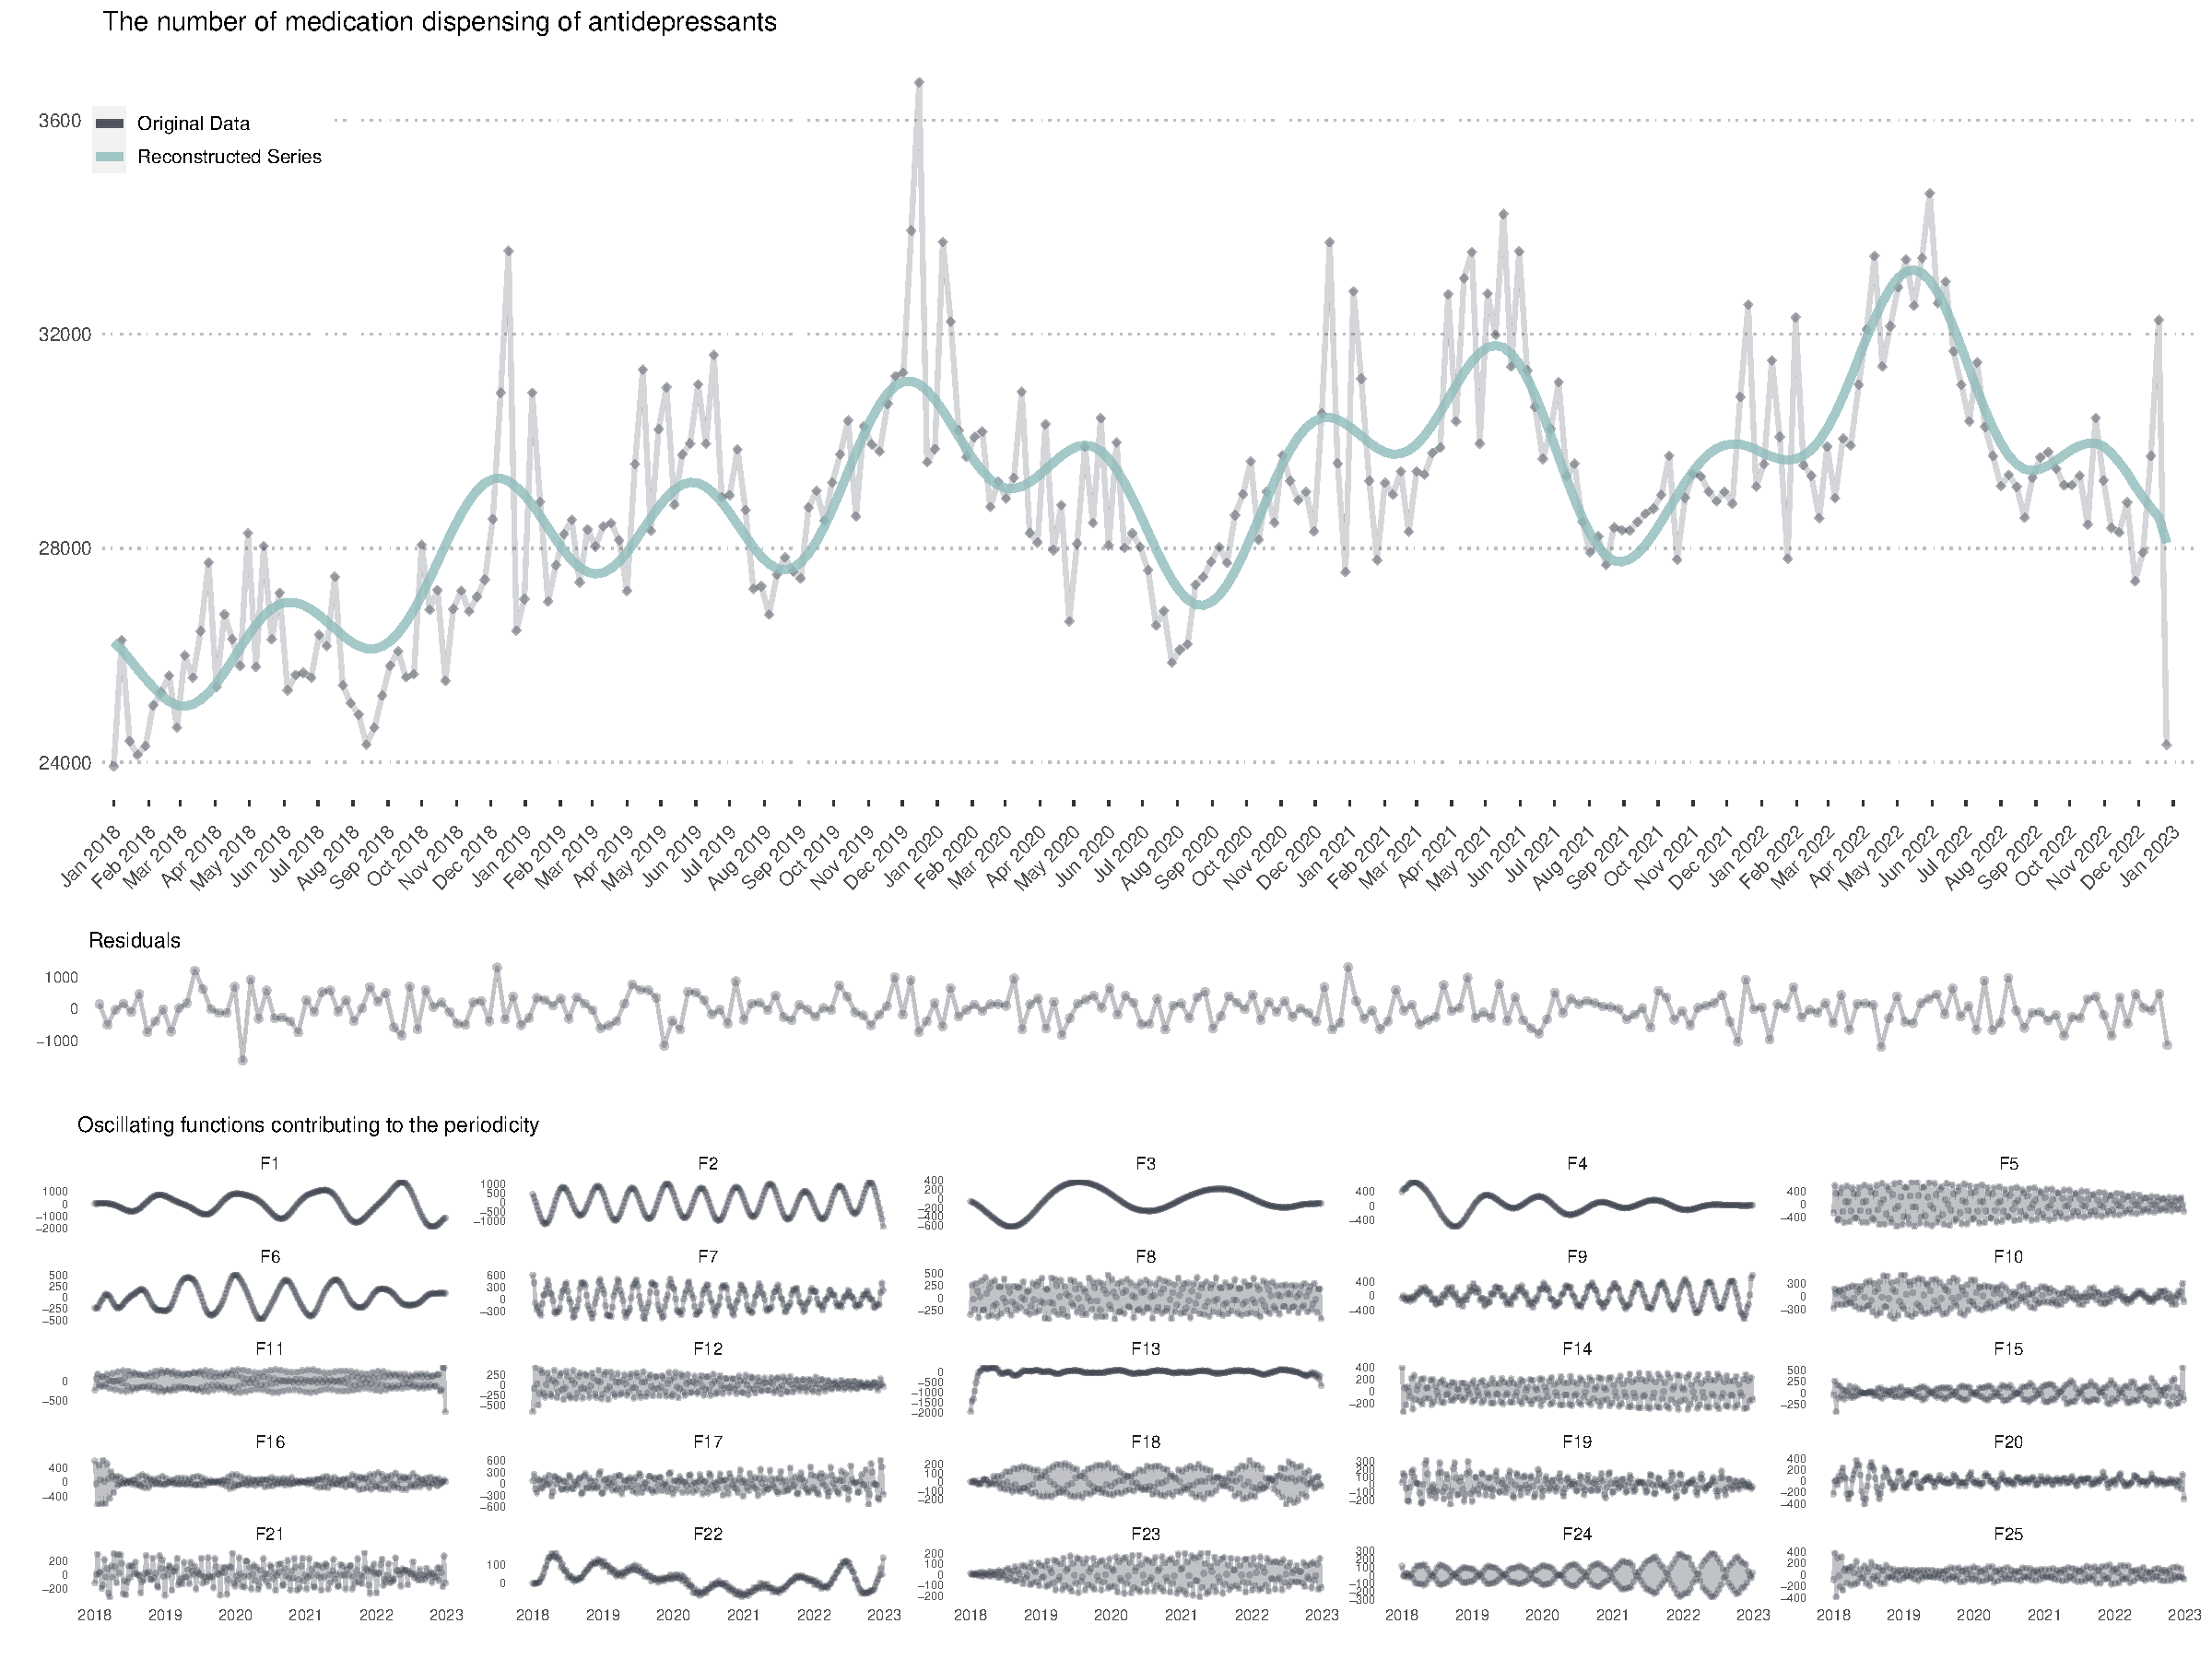
\includegraphics[width=1\linewidth,height=\textheight,keepaspectratio]{article_files/figure-pdf/fig-ssa-1.pdf}

}

\caption{\label{fig-ssa}Time-series decomposition of antidepressants
dispensing data using singular spectrum analysis-based approach}

\end{figure}%

\subsection{Eigenvector centrality
measures}\label{eigenvector-centrality-measures}

Seven medication classes exhibited high centrality, as shown in
Figure~\ref{fig-hi-eigen} and Table~\ref{tbl-desc}. Notably, highly
dispensed medications generally had high eigenvector centrality,
consistent with the theoretical expectations from
Equation~\ref{eq-eigen-centrality}. However, this relationship was not
strictly proportional. For example, although antidepressants had a
higher number of prescription dispensed compared to medications for the
respiratory system (6,108,776 vs 5,492,900), they exhibited lower
eigenvector centrality (9.48e-02 {[}SD: 2.24e-03{]} vs 9.53e-02 {[}SD:
2.21e-03{]}). A similar pattern was observed for anxiolytics, which had
more dispensing than analgesics (2,644,309 vs 2,557,528) but lower
eigenvector centrality (5.25e-02 {[}SD: 4.13e-03{]} vs 5.84e-02 {[}SD:
3.94e-03{]}). These discrepancies show that higher centrality scores
capture more than just a high dispensing volume.

\global\setlength{\Oldarrayrulewidth}{\arrayrulewidth}

\global\setlength{\Oldtabcolsep}{\tabcolsep}

\setlength{\tabcolsep}{0pt}

\renewcommand*{\arraystretch}{1}



\providecommand{\ascline}[3]{\noalign{\global\arrayrulewidth #1}\arrayrulecolor[HTML]{#2}\cline{#3}}

\begin{longtable}[c]{|p{1.57in}|p{0.75in}|p{1.16in}|p{1.16in}|p{1.16in}}

\caption{\label{tbl-desc}Descriptive statistics of dispensing data from
2018 to 2022, ordered by Eigenvector centrality}

\tabularnewline

\ascline{1.5pt}{666666}{1-5}

\multicolumn{2}{>{\raggedright}m{\dimexpr 2.32in+2\tabcolsep}}{\textcolor[HTML]{000000}{\fontsize{7}{7}\selectfont{\global\setmainfont{DejaVu Sans}{}}}} & \multicolumn{3}{>{\centering}m{\dimexpr 3.49in+4\tabcolsep}}{\textcolor[HTML]{000000}{\fontsize{7}{7}\selectfont{\global\setmainfont{DejaVu Sans}{Mean\ [SD]}}}} \\

\ascline{1.5pt}{666666}{1-5}



\multicolumn{1}{>{\raggedright}m{\dimexpr 1.57in+0\tabcolsep}}{\textcolor[HTML]{000000}{\fontsize{7}{7}\selectfont{\global\setmainfont{DejaVu Sans}{}}}} & \multicolumn{1}{>{\centering}m{\dimexpr 0.75in+0\tabcolsep}}{\textcolor[HTML]{000000}{\fontsize{7}{7}\selectfont{\global\setmainfont{DejaVu Sans}{Dispensing}}}} & \multicolumn{1}{>{\centering}m{\dimexpr 1.16in+0\tabcolsep}}{\textcolor[HTML]{000000}{\fontsize{7}{7}\selectfont{\global\setmainfont{DejaVu Sans}{Centrality}}}} & \multicolumn{1}{>{\centering}m{\dimexpr 1.16in+0\tabcolsep}}{\textcolor[HTML]{000000}{\fontsize{7}{7}\selectfont{\global\setmainfont{DejaVu Sans}{DDD}}}\textcolor[HTML]{000000}{\fontsize{7}{7}\selectfont{\global\setmainfont{DejaVu Sans}{\textsuperscript{1}}}}} & \multicolumn{1}{>{\centering}m{\dimexpr 1.16in+0\tabcolsep}}{\textcolor[HTML]{000000}{\fontsize{7}{7}\selectfont{\global\setmainfont{DejaVu Sans}{Weight}}}\textcolor[HTML]{000000}{\fontsize{7}{7}\selectfont{\global\setmainfont{DejaVu Sans}{\textsuperscript{2}}}}} \\

\ascline{1.5pt}{666666}{1-5}\endfirsthead 

\ascline{1.5pt}{666666}{1-5}

\multicolumn{2}{>{\raggedright}m{\dimexpr 2.32in+2\tabcolsep}}{\textcolor[HTML]{000000}{\fontsize{7}{7}\selectfont{\global\setmainfont{DejaVu Sans}{}}}} & \multicolumn{3}{>{\centering}m{\dimexpr 3.49in+4\tabcolsep}}{\textcolor[HTML]{000000}{\fontsize{7}{7}\selectfont{\global\setmainfont{DejaVu Sans}{Mean\ [SD]}}}} \\

\ascline{1.5pt}{666666}{1-5}



\multicolumn{1}{>{\raggedright}m{\dimexpr 1.57in+0\tabcolsep}}{\textcolor[HTML]{000000}{\fontsize{7}{7}\selectfont{\global\setmainfont{DejaVu Sans}{}}}} & \multicolumn{1}{>{\centering}m{\dimexpr 0.75in+0\tabcolsep}}{\textcolor[HTML]{000000}{\fontsize{7}{7}\selectfont{\global\setmainfont{DejaVu Sans}{Dispensing}}}} & \multicolumn{1}{>{\centering}m{\dimexpr 1.16in+0\tabcolsep}}{\textcolor[HTML]{000000}{\fontsize{7}{7}\selectfont{\global\setmainfont{DejaVu Sans}{Centrality}}}} & \multicolumn{1}{>{\centering}m{\dimexpr 1.16in+0\tabcolsep}}{\textcolor[HTML]{000000}{\fontsize{7}{7}\selectfont{\global\setmainfont{DejaVu Sans}{DDD}}}\textcolor[HTML]{000000}{\fontsize{7}{7}\selectfont{\global\setmainfont{DejaVu Sans}{\textsuperscript{1}}}}} & \multicolumn{1}{>{\centering}m{\dimexpr 1.16in+0\tabcolsep}}{\textcolor[HTML]{000000}{\fontsize{7}{7}\selectfont{\global\setmainfont{DejaVu Sans}{Weight}}}\textcolor[HTML]{000000}{\fontsize{7}{7}\selectfont{\global\setmainfont{DejaVu Sans}{\textsuperscript{2}}}}} \\

\ascline{1.5pt}{666666}{1-5}\endhead



\multicolumn{1}{>{\raggedright}m{\dimexpr 1.57in+0\tabcolsep}}{\textcolor[HTML]{000000}{\fontsize{7}{7}\selectfont{\global\setmainfont{DejaVu Sans}{Alimentary\ and\ metabolism}}}} & \multicolumn{1}{>{\centering}m{\dimexpr 0.75in+0\tabcolsep}}{\textcolor[HTML]{000000}{\fontsize{7}{7}\selectfont{\global\setmainfont{DejaVu Sans}{11,512,424}}}} & \multicolumn{1}{>{\centering}m{\dimexpr 1.16in+0\tabcolsep}}{\textcolor[HTML]{000000}{\fontsize{7}{7}\selectfont{\global\setmainfont{DejaVu Sans}{1.59e-01\ [5.00e-03]}}}} & \multicolumn{1}{>{\centering}m{\dimexpr 1.16in+0\tabcolsep}}{\textcolor[HTML]{000000}{\fontsize{7}{7}\selectfont{\global\setmainfont{DejaVu Sans}{5.97e-01\ [3.26e-01]}}}} & \multicolumn{1}{>{\centering}m{\dimexpr 1.16in+0\tabcolsep}}{\textcolor[HTML]{000000}{\fontsize{7}{7}\selectfont{\global\setmainfont{DejaVu Sans}{7.28e-01\ [2.06e-01]}}}} \\





\multicolumn{1}{>{\raggedright}m{\dimexpr 1.57in+0\tabcolsep}}{\textcolor[HTML]{000000}{\fontsize{7}{7}\selectfont{\global\setmainfont{DejaVu Sans}{Cardiovascular}}}} & \multicolumn{1}{>{\centering}m{\dimexpr 0.75in+0\tabcolsep}}{\textcolor[HTML]{000000}{\fontsize{7}{7}\selectfont{\global\setmainfont{DejaVu Sans}{9,778,030}}}} & \multicolumn{1}{>{\centering}m{\dimexpr 1.16in+0\tabcolsep}}{\textcolor[HTML]{000000}{\fontsize{7}{7}\selectfont{\global\setmainfont{DejaVu Sans}{1.50e-01\ [6.87e-03]}}}} & \multicolumn{1}{>{\centering}m{\dimexpr 1.16in+0\tabcolsep}}{\textcolor[HTML]{000000}{\fontsize{7}{7}\selectfont{\global\setmainfont{DejaVu Sans}{5.38e-01\ [3.05e-01]}}}} & \multicolumn{1}{>{\centering}m{\dimexpr 1.16in+0\tabcolsep}}{\textcolor[HTML]{000000}{\fontsize{7}{7}\selectfont{\global\setmainfont{DejaVu Sans}{6.92e-01\ [2.00e-01]}}}} \\





\multicolumn{1}{>{\raggedright}m{\dimexpr 1.57in+0\tabcolsep}}{\textcolor[HTML]{000000}{\fontsize{7}{7}\selectfont{\global\setmainfont{DejaVu Sans}{Respiratory}}}} & \multicolumn{1}{>{\centering}m{\dimexpr 0.75in+0\tabcolsep}}{\textcolor[HTML]{000000}{\fontsize{7}{7}\selectfont{\global\setmainfont{DejaVu Sans}{5,492,900}}}} & \multicolumn{1}{>{\centering}m{\dimexpr 1.16in+0\tabcolsep}}{\textcolor[HTML]{000000}{\fontsize{7}{7}\selectfont{\global\setmainfont{DejaVu Sans}{9.53e-02\ [2.21e-03]}}}} & \multicolumn{1}{>{\centering}m{\dimexpr 1.16in+0\tabcolsep}}{\textcolor[HTML]{000000}{\fontsize{7}{7}\selectfont{\global\setmainfont{DejaVu Sans}{6.55e-01\ [3.25e-01]}}}} & \multicolumn{1}{>{\centering}m{\dimexpr 1.16in+0\tabcolsep}}{\textcolor[HTML]{000000}{\fontsize{7}{7}\selectfont{\global\setmainfont{DejaVu Sans}{7.70e-01\ [2.15e-01]}}}} \\





\multicolumn{1}{>{\raggedright}m{\dimexpr 1.57in+0\tabcolsep}}{\textcolor[HTML]{000000}{\fontsize{7}{7}\selectfont{\global\setmainfont{DejaVu Sans}{Antidepressants}}}} & \multicolumn{1}{>{\centering}m{\dimexpr 0.75in+0\tabcolsep}}{\textcolor[HTML]{000000}{\fontsize{7}{7}\selectfont{\global\setmainfont{DejaVu Sans}{6,108,776}}}} & \multicolumn{1}{>{\centering}m{\dimexpr 1.16in+0\tabcolsep}}{\textcolor[HTML]{000000}{\fontsize{7}{7}\selectfont{\global\setmainfont{DejaVu Sans}{9.48e-02\ [2.24e-03]}}}} & \multicolumn{1}{>{\centering}m{\dimexpr 1.16in+0\tabcolsep}}{\textcolor[HTML]{000000}{\fontsize{7}{7}\selectfont{\global\setmainfont{DejaVu Sans}{5.36e-01\ [3.09e-01]}}}} & \multicolumn{1}{>{\centering}m{\dimexpr 1.16in+0\tabcolsep}}{\textcolor[HTML]{000000}{\fontsize{7}{7}\selectfont{\global\setmainfont{DejaVu Sans}{6.92e-01\ [2.03e-01]}}}} \\





\multicolumn{1}{>{\raggedright}m{\dimexpr 1.57in+0\tabcolsep}}{\textcolor[HTML]{000000}{\fontsize{7}{7}\selectfont{\global\setmainfont{DejaVu Sans}{Blood}}}} & \multicolumn{1}{>{\centering}m{\dimexpr 0.75in+0\tabcolsep}}{\textcolor[HTML]{000000}{\fontsize{7}{7}\selectfont{\global\setmainfont{DejaVu Sans}{2,908,944}}}} & \multicolumn{1}{>{\centering}m{\dimexpr 1.16in+0\tabcolsep}}{\textcolor[HTML]{000000}{\fontsize{7}{7}\selectfont{\global\setmainfont{DejaVu Sans}{8.87e-02\ [5.64e-03]}}}} & \multicolumn{1}{>{\centering}m{\dimexpr 1.16in+0\tabcolsep}}{\textcolor[HTML]{000000}{\fontsize{7}{7}\selectfont{\global\setmainfont{DejaVu Sans}{6.93e-01\ [3.91e-01]}}}} & \multicolumn{1}{>{\centering}m{\dimexpr 1.16in+0\tabcolsep}}{\textcolor[HTML]{000000}{\fontsize{7}{7}\selectfont{\global\setmainfont{DejaVu Sans}{7.78e-01\ [2.13e-01]}}}} \\





\multicolumn{1}{>{\raggedright}m{\dimexpr 1.57in+0\tabcolsep}}{\textcolor[HTML]{000000}{\fontsize{7}{7}\selectfont{\global\setmainfont{DejaVu Sans}{Analgesics}}}} & \multicolumn{1}{>{\centering}m{\dimexpr 0.75in+0\tabcolsep}}{\textcolor[HTML]{000000}{\fontsize{7}{7}\selectfont{\global\setmainfont{DejaVu Sans}{2,557,528}}}} & \multicolumn{1}{>{\centering}m{\dimexpr 1.16in+0\tabcolsep}}{\textcolor[HTML]{000000}{\fontsize{7}{7}\selectfont{\global\setmainfont{DejaVu Sans}{5.84e-02\ [3.94e-03]}}}} & \multicolumn{1}{>{\centering}m{\dimexpr 1.16in+0\tabcolsep}}{\textcolor[HTML]{000000}{\fontsize{7}{7}\selectfont{\global\setmainfont{DejaVu Sans}{4.23e-01\ [2.60e-01]}}}} & \multicolumn{1}{>{\centering}m{\dimexpr 1.16in+0\tabcolsep}}{\textcolor[HTML]{000000}{\fontsize{7}{7}\selectfont{\global\setmainfont{DejaVu Sans}{6.16e-01\ [1.66e-01]}}}} \\





\multicolumn{1}{>{\raggedright}m{\dimexpr 1.57in+0\tabcolsep}}{\textcolor[HTML]{000000}{\fontsize{7}{7}\selectfont{\global\setmainfont{DejaVu Sans}{Anxiolytics}}}} & \multicolumn{1}{>{\centering}m{\dimexpr 0.75in+0\tabcolsep}}{\textcolor[HTML]{000000}{\fontsize{7}{7}\selectfont{\global\setmainfont{DejaVu Sans}{2,644,309}}}} & \multicolumn{1}{>{\centering}m{\dimexpr 1.16in+0\tabcolsep}}{\textcolor[HTML]{000000}{\fontsize{7}{7}\selectfont{\global\setmainfont{DejaVu Sans}{5.25e-02\ [4.13e-03]}}}} & \multicolumn{1}{>{\centering}m{\dimexpr 1.16in+0\tabcolsep}}{\textcolor[HTML]{000000}{\fontsize{7}{7}\selectfont{\global\setmainfont{DejaVu Sans}{4.63e-01\ [2.88e-01]}}}} & \multicolumn{1}{>{\centering}m{\dimexpr 1.16in+0\tabcolsep}}{\textcolor[HTML]{000000}{\fontsize{7}{7}\selectfont{\global\setmainfont{DejaVu Sans}{6.35e-01\ [1.73e-01]}}}} \\





\multicolumn{1}{>{\raggedright}m{\dimexpr 1.57in+0\tabcolsep}}{\textcolor[HTML]{000000}{\fontsize{7}{7}\selectfont{\global\setmainfont{DejaVu Sans}{Dermatologicals}}}} & \multicolumn{1}{>{\centering}m{\dimexpr 0.75in+0\tabcolsep}}{\textcolor[HTML]{000000}{\fontsize{7}{7}\selectfont{\global\setmainfont{DejaVu Sans}{2,086,095}}}} & \multicolumn{1}{>{\centering}m{\dimexpr 1.16in+0\tabcolsep}}{\textcolor[HTML]{000000}{\fontsize{7}{7}\selectfont{\global\setmainfont{DejaVu Sans}{4.03e-02\ [1.34e-03]}}}} & \multicolumn{1}{>{\centering}m{\dimexpr 1.16in+0\tabcolsep}}{\textcolor[HTML]{000000}{\fontsize{7}{7}\selectfont{\global\setmainfont{DejaVu Sans}{8.08e-01\ [3.39e-01]}}}} & \multicolumn{1}{>{\centering}m{\dimexpr 1.16in+0\tabcolsep}}{\textcolor[HTML]{000000}{\fontsize{7}{7}\selectfont{\global\setmainfont{DejaVu Sans}{8.62e-01\ [2.09e-01]}}}} \\





\multicolumn{1}{>{\raggedright}m{\dimexpr 1.57in+0\tabcolsep}}{\textcolor[HTML]{000000}{\fontsize{7}{7}\selectfont{\global\setmainfont{DejaVu Sans}{Musculoskeletal}}}} & \multicolumn{1}{>{\centering}m{\dimexpr 0.75in+0\tabcolsep}}{\textcolor[HTML]{000000}{\fontsize{7}{7}\selectfont{\global\setmainfont{DejaVu Sans}{1,449,535}}}} & \multicolumn{1}{>{\centering}m{\dimexpr 1.16in+0\tabcolsep}}{\textcolor[HTML]{000000}{\fontsize{7}{7}\selectfont{\global\setmainfont{DejaVu Sans}{3.95e-02\ [1.52e-03]}}}} & \multicolumn{1}{>{\centering}m{\dimexpr 1.16in+0\tabcolsep}}{\textcolor[HTML]{000000}{\fontsize{7}{7}\selectfont{\global\setmainfont{DejaVu Sans}{5.59e-01\ [3.26e-01]}}}} & \multicolumn{1}{>{\centering}m{\dimexpr 1.16in+0\tabcolsep}}{\textcolor[HTML]{000000}{\fontsize{7}{7}\selectfont{\global\setmainfont{DejaVu Sans}{7.10e-01\ [2.11e-01]}}}} \\





\multicolumn{1}{>{\raggedright}m{\dimexpr 1.57in+0\tabcolsep}}{\textcolor[HTML]{000000}{\fontsize{7}{7}\selectfont{\global\setmainfont{DejaVu Sans}{Systemic\ hormonal}}}} & \multicolumn{1}{>{\centering}m{\dimexpr 0.75in+0\tabcolsep}}{\textcolor[HTML]{000000}{\fontsize{7}{7}\selectfont{\global\setmainfont{DejaVu Sans}{1,602,716}}}} & \multicolumn{1}{>{\centering}m{\dimexpr 1.16in+0\tabcolsep}}{\textcolor[HTML]{000000}{\fontsize{7}{7}\selectfont{\global\setmainfont{DejaVu Sans}{3.80e-02\ [1.71e-03]}}}} & \multicolumn{1}{>{\centering}m{\dimexpr 1.16in+0\tabcolsep}}{\textcolor[HTML]{000000}{\fontsize{7}{7}\selectfont{\global\setmainfont{DejaVu Sans}{4.97e-01\ [2.76e-01]}}}} & \multicolumn{1}{>{\centering}m{\dimexpr 1.16in+0\tabcolsep}}{\textcolor[HTML]{000000}{\fontsize{7}{7}\selectfont{\global\setmainfont{DejaVu Sans}{6.55e-01\ [1.66e-01]}}}} \\





\multicolumn{1}{>{\raggedright}m{\dimexpr 1.57in+0\tabcolsep}}{\textcolor[HTML]{000000}{\fontsize{7}{7}\selectfont{\global\setmainfont{DejaVu Sans}{Antipsychotics}}}} & \multicolumn{1}{>{\centering}m{\dimexpr 0.75in+0\tabcolsep}}{\textcolor[HTML]{000000}{\fontsize{7}{7}\selectfont{\global\setmainfont{DejaVu Sans}{2,473,609}}}} & \multicolumn{1}{>{\centering}m{\dimexpr 1.16in+0\tabcolsep}}{\textcolor[HTML]{000000}{\fontsize{7}{7}\selectfont{\global\setmainfont{DejaVu Sans}{3.70e-02\ [3.20e-03]}}}} & \multicolumn{1}{>{\centering}m{\dimexpr 1.16in+0\tabcolsep}}{\textcolor[HTML]{000000}{\fontsize{7}{7}\selectfont{\global\setmainfont{DejaVu Sans}{4.04e-01\ [2.65e-01]}}}} & \multicolumn{1}{>{\centering}m{\dimexpr 1.16in+0\tabcolsep}}{\textcolor[HTML]{000000}{\fontsize{7}{7}\selectfont{\global\setmainfont{DejaVu Sans}{6.10e-01\ [1.69e-01]}}}} \\





\multicolumn{1}{>{\raggedright}m{\dimexpr 1.57in+0\tabcolsep}}{\textcolor[HTML]{000000}{\fontsize{7}{7}\selectfont{\global\setmainfont{DejaVu Sans}{Genitourinary}}}} & \multicolumn{1}{>{\centering}m{\dimexpr 0.75in+0\tabcolsep}}{\textcolor[HTML]{000000}{\fontsize{7}{7}\selectfont{\global\setmainfont{DejaVu Sans}{2,099,833}}}} & \multicolumn{1}{>{\centering}m{\dimexpr 1.16in+0\tabcolsep}}{\textcolor[HTML]{000000}{\fontsize{7}{7}\selectfont{\global\setmainfont{DejaVu Sans}{3.39e-02\ [9.53e-04]}}}} & \multicolumn{1}{>{\centering}m{\dimexpr 1.16in+0\tabcolsep}}{\textcolor[HTML]{000000}{\fontsize{7}{7}\selectfont{\global\setmainfont{DejaVu Sans}{7.46e-01\ [3.69e-01]}}}} & \multicolumn{1}{>{\centering}m{\dimexpr 1.16in+0\tabcolsep}}{\textcolor[HTML]{000000}{\fontsize{7}{7}\selectfont{\global\setmainfont{DejaVu Sans}{8.29e-01\ [2.12e-01]}}}} \\





\multicolumn{1}{>{\raggedright}m{\dimexpr 1.57in+0\tabcolsep}}{\textcolor[HTML]{000000}{\fontsize{7}{7}\selectfont{\global\setmainfont{DejaVu Sans}{Hypnotics\ and\ sedatives}}}} & \multicolumn{1}{>{\centering}m{\dimexpr 0.75in+0\tabcolsep}}{\textcolor[HTML]{000000}{\fontsize{7}{7}\selectfont{\global\setmainfont{DejaVu Sans}{1,467,752}}}} & \multicolumn{1}{>{\centering}m{\dimexpr 1.16in+0\tabcolsep}}{\textcolor[HTML]{000000}{\fontsize{7}{7}\selectfont{\global\setmainfont{DejaVu Sans}{3.37e-02\ [3.23e-03]}}}} & \multicolumn{1}{>{\centering}m{\dimexpr 1.16in+0\tabcolsep}}{\textcolor[HTML]{000000}{\fontsize{7}{7}\selectfont{\global\setmainfont{DejaVu Sans}{6.31e-01\ [3.16e-01]}}}} & \multicolumn{1}{>{\centering}m{\dimexpr 1.16in+0\tabcolsep}}{\textcolor[HTML]{000000}{\fontsize{7}{7}\selectfont{\global\setmainfont{DejaVu Sans}{7.49e-01\ [2.09e-01]}}}} \\





\multicolumn{1}{>{\raggedright}m{\dimexpr 1.57in+0\tabcolsep}}{\textcolor[HTML]{000000}{\fontsize{7}{7}\selectfont{\global\setmainfont{DejaVu Sans}{Systemic\ anti-infectives}}}} & \multicolumn{1}{>{\centering}m{\dimexpr 0.75in+0\tabcolsep}}{\textcolor[HTML]{000000}{\fontsize{7}{7}\selectfont{\global\setmainfont{DejaVu Sans}{734,706}}}} & \multicolumn{1}{>{\centering}m{\dimexpr 1.16in+0\tabcolsep}}{\textcolor[HTML]{000000}{\fontsize{7}{7}\selectfont{\global\setmainfont{DejaVu Sans}{2.07e-02\ [1.47e-03]}}}} & \multicolumn{1}{>{\centering}m{\dimexpr 1.16in+0\tabcolsep}}{\textcolor[HTML]{000000}{\fontsize{7}{7}\selectfont{\global\setmainfont{DejaVu Sans}{6.34e-01\ [3.23e-01]}}}} & \multicolumn{1}{>{\centering}m{\dimexpr 1.16in+0\tabcolsep}}{\textcolor[HTML]{000000}{\fontsize{7}{7}\selectfont{\global\setmainfont{DejaVu Sans}{7.64e-01\ [2.21e-01]}}}} \\





\multicolumn{1}{>{\raggedright}m{\dimexpr 1.57in+0\tabcolsep}}{\textcolor[HTML]{000000}{\fontsize{7}{7}\selectfont{\global\setmainfont{DejaVu Sans}{Antiepileptics}}}} & \multicolumn{1}{>{\centering}m{\dimexpr 0.75in+0\tabcolsep}}{\textcolor[HTML]{000000}{\fontsize{7}{7}\selectfont{\global\setmainfont{DejaVu Sans}{1,078,266}}}} & \multicolumn{1}{>{\centering}m{\dimexpr 1.16in+0\tabcolsep}}{\textcolor[HTML]{000000}{\fontsize{7}{7}\selectfont{\global\setmainfont{DejaVu Sans}{2.06e-02\ [2.73e-03]}}}} & \multicolumn{1}{>{\centering}m{\dimexpr 1.16in+0\tabcolsep}}{\textcolor[HTML]{000000}{\fontsize{7}{7}\selectfont{\global\setmainfont{DejaVu Sans}{4.29e-01\ [2.52e-01]}}}} & \multicolumn{1}{>{\centering}m{\dimexpr 1.16in+0\tabcolsep}}{\textcolor[HTML]{000000}{\fontsize{7}{7}\selectfont{\global\setmainfont{DejaVu Sans}{6.25e-01\ [1.66e-01]}}}} \\





\multicolumn{1}{>{\raggedright}m{\dimexpr 1.57in+0\tabcolsep}}{\textcolor[HTML]{000000}{\fontsize{7}{7}\selectfont{\global\setmainfont{DejaVu Sans}{Antineoplastics}}}} & \multicolumn{1}{>{\centering}m{\dimexpr 0.75in+0\tabcolsep}}{\textcolor[HTML]{000000}{\fontsize{7}{7}\selectfont{\global\setmainfont{DejaVu Sans}{449,030}}}} & \multicolumn{1}{>{\centering}m{\dimexpr 1.16in+0\tabcolsep}}{\textcolor[HTML]{000000}{\fontsize{7}{7}\selectfont{\global\setmainfont{DejaVu Sans}{1.03e-02\ [4.68e-04]}}}} & \multicolumn{1}{>{\centering}m{\dimexpr 1.16in+0\tabcolsep}}{\textcolor[HTML]{000000}{\fontsize{7}{7}\selectfont{\global\setmainfont{DejaVu Sans}{6.13e-01\ [3.01e-01]}}}} & \multicolumn{1}{>{\centering}m{\dimexpr 1.16in+0\tabcolsep}}{\textcolor[HTML]{000000}{\fontsize{7}{7}\selectfont{\global\setmainfont{DejaVu Sans}{7.49e-01\ [2.05e-01]}}}} \\





\multicolumn{1}{>{\raggedright}m{\dimexpr 1.57in+0\tabcolsep}}{\textcolor[HTML]{000000}{\fontsize{7}{7}\selectfont{\global\setmainfont{DejaVu Sans}{Other\ nervous\ system\ drugs}}}} & \multicolumn{1}{>{\centering}m{\dimexpr 0.75in+0\tabcolsep}}{\textcolor[HTML]{000000}{\fontsize{7}{7}\selectfont{\global\setmainfont{DejaVu Sans}{362,624}}}} & \multicolumn{1}{>{\centering}m{\dimexpr 1.16in+0\tabcolsep}}{\textcolor[HTML]{000000}{\fontsize{7}{7}\selectfont{\global\setmainfont{DejaVu Sans}{8.79e-03\ [1.08e-03]}}}} & \multicolumn{1}{>{\centering}m{\dimexpr 1.16in+0\tabcolsep}}{\textcolor[HTML]{000000}{\fontsize{7}{7}\selectfont{\global\setmainfont{DejaVu Sans}{5.23e-01\ [3.16e-01]}}}} & \multicolumn{1}{>{\centering}m{\dimexpr 1.16in+0\tabcolsep}}{\textcolor[HTML]{000000}{\fontsize{7}{7}\selectfont{\global\setmainfont{DejaVu Sans}{6.78e-01\ [1.93e-01]}}}} \\





\multicolumn{1}{>{\raggedright}m{\dimexpr 1.57in+0\tabcolsep}}{\textcolor[HTML]{000000}{\fontsize{7}{7}\selectfont{\global\setmainfont{DejaVu Sans}{Antiparkinson}}}} & \multicolumn{1}{>{\centering}m{\dimexpr 0.75in+0\tabcolsep}}{\textcolor[HTML]{000000}{\fontsize{7}{7}\selectfont{\global\setmainfont{DejaVu Sans}{306,541}}}} & \multicolumn{1}{>{\centering}m{\dimexpr 1.16in+0\tabcolsep}}{\textcolor[HTML]{000000}{\fontsize{7}{7}\selectfont{\global\setmainfont{DejaVu Sans}{6.17e-03\ [5.64e-04]}}}} & \multicolumn{1}{>{\centering}m{\dimexpr 1.16in+0\tabcolsep}}{\textcolor[HTML]{000000}{\fontsize{7}{7}\selectfont{\global\setmainfont{DejaVu Sans}{3.53e-01\ [2.21e-01]}}}} & \multicolumn{1}{>{\centering}m{\dimexpr 1.16in+0\tabcolsep}}{\textcolor[HTML]{000000}{\fontsize{7}{7}\selectfont{\global\setmainfont{DejaVu Sans}{5.74e-01\ [1.37e-01]}}}} \\





\multicolumn{1}{>{\raggedright}m{\dimexpr 1.57in+0\tabcolsep}}{\textcolor[HTML]{000000}{\fontsize{7}{7}\selectfont{\global\setmainfont{DejaVu Sans}{Psychostimulants}}}} & \multicolumn{1}{>{\centering}m{\dimexpr 0.75in+0\tabcolsep}}{\textcolor[HTML]{000000}{\fontsize{7}{7}\selectfont{\global\setmainfont{DejaVu Sans}{459,207}}}} & \multicolumn{1}{>{\centering}m{\dimexpr 1.16in+0\tabcolsep}}{\textcolor[HTML]{000000}{\fontsize{7}{7}\selectfont{\global\setmainfont{DejaVu Sans}{5.56e-03\ [8.26e-04]}}}} & \multicolumn{1}{>{\centering}m{\dimexpr 1.16in+0\tabcolsep}}{\textcolor[HTML]{000000}{\fontsize{7}{7}\selectfont{\global\setmainfont{DejaVu Sans}{5.20e-01\ [3.13e-01]}}}} & \multicolumn{1}{>{\centering}m{\dimexpr 1.16in+0\tabcolsep}}{\textcolor[HTML]{000000}{\fontsize{7}{7}\selectfont{\global\setmainfont{DejaVu Sans}{6.74e-01\ [1.90e-01]}}}} \\





\multicolumn{1}{>{\raggedright}m{\dimexpr 1.57in+0\tabcolsep}}{\textcolor[HTML]{000000}{\fontsize{7}{7}\selectfont{\global\setmainfont{DejaVu Sans}{Sensory}}}} & \multicolumn{1}{>{\centering}m{\dimexpr 0.75in+0\tabcolsep}}{\textcolor[HTML]{000000}{\fontsize{7}{7}\selectfont{\global\setmainfont{DejaVu Sans}{196,513}}}} & \multicolumn{1}{>{\centering}m{\dimexpr 1.16in+0\tabcolsep}}{\textcolor[HTML]{000000}{\fontsize{7}{7}\selectfont{\global\setmainfont{DejaVu Sans}{3.36e-03\ [5.91e-04]}}}} & \multicolumn{1}{>{\centering}m{\dimexpr 1.16in+0\tabcolsep}}{\textcolor[HTML]{000000}{\fontsize{7}{7}\selectfont{\global\setmainfont{DejaVu Sans}{4.66e-01\ [2.87e-01]}}}} & \multicolumn{1}{>{\centering}m{\dimexpr 1.16in+0\tabcolsep}}{\textcolor[HTML]{000000}{\fontsize{7}{7}\selectfont{\global\setmainfont{DejaVu Sans}{6.37e-01\ [1.80e-01]}}}} \\





\multicolumn{1}{>{\raggedright}m{\dimexpr 1.57in+0\tabcolsep}}{\textcolor[HTML]{000000}{\fontsize{7}{7}\selectfont{\global\setmainfont{DejaVu Sans}{Antiparasitics}}}} & \multicolumn{1}{>{\centering}m{\dimexpr 0.75in+0\tabcolsep}}{\textcolor[HTML]{000000}{\fontsize{7}{7}\selectfont{\global\setmainfont{DejaVu Sans}{88,760}}}} & \multicolumn{1}{>{\centering}m{\dimexpr 1.16in+0\tabcolsep}}{\textcolor[HTML]{000000}{\fontsize{7}{7}\selectfont{\global\setmainfont{DejaVu Sans}{1.61e-03\ [1.20e-04]}}}} & \multicolumn{1}{>{\centering}m{\dimexpr 1.16in+0\tabcolsep}}{\textcolor[HTML]{000000}{\fontsize{7}{7}\selectfont{\global\setmainfont{DejaVu Sans}{5.24e-01\ [2.53e-01]}}}} & \multicolumn{1}{>{\centering}m{\dimexpr 1.16in+0\tabcolsep}}{\textcolor[HTML]{000000}{\fontsize{7}{7}\selectfont{\global\setmainfont{DejaVu Sans}{6.72e-01\ [1.65e-01]}}}} \\





\multicolumn{1}{>{\raggedright}m{\dimexpr 1.57in+0\tabcolsep}}{\textcolor[HTML]{000000}{\fontsize{7}{7}\selectfont{\global\setmainfont{DejaVu Sans}{Anesthetic}}}} & \multicolumn{1}{>{\centering}m{\dimexpr 0.75in+0\tabcolsep}}{\textcolor[HTML]{000000}{\fontsize{7}{7}\selectfont{\global\setmainfont{DejaVu Sans}{39,455}}}} & \multicolumn{1}{>{\centering}m{\dimexpr 1.16in+0\tabcolsep}}{\textcolor[HTML]{000000}{\fontsize{7}{7}\selectfont{\global\setmainfont{DejaVu Sans}{1.15e-03\ [2.15e-04]}}}} & \multicolumn{1}{>{\centering}m{\dimexpr 1.16in+0\tabcolsep}}{\textcolor[HTML]{000000}{\fontsize{7}{7}\selectfont{\global\setmainfont{DejaVu Sans}{6.45e-01\ [4.47e-01]}}}} & \multicolumn{1}{>{\centering}m{\dimexpr 1.16in+0\tabcolsep}}{\textcolor[HTML]{000000}{\fontsize{7}{7}\selectfont{\global\setmainfont{DejaVu Sans}{7.39e-01\ [2.31e-01]}}}} \\





\multicolumn{1}{>{\raggedright}m{\dimexpr 1.57in+0\tabcolsep}}{\textcolor[HTML]{000000}{\fontsize{7}{7}\selectfont{\global\setmainfont{DejaVu Sans}{Others}}}} & \multicolumn{1}{>{\centering}m{\dimexpr 0.75in+0\tabcolsep}}{\textcolor[HTML]{000000}{\fontsize{7}{7}\selectfont{\global\setmainfont{DejaVu Sans}{18,157}}}} & \multicolumn{1}{>{\centering}m{\dimexpr 1.16in+0\tabcolsep}}{\textcolor[HTML]{000000}{\fontsize{7}{7}\selectfont{\global\setmainfont{DejaVu Sans}{2.94e-04\ [4.86e-05]}}}} & \multicolumn{1}{>{\centering}m{\dimexpr 1.16in+0\tabcolsep}}{\textcolor[HTML]{000000}{\fontsize{7}{7}\selectfont{\global\setmainfont{DejaVu Sans}{4.55e-01\ [2.73e-01]}}}} & \multicolumn{1}{>{\centering}m{\dimexpr 1.16in+0\tabcolsep}}{\textcolor[HTML]{000000}{\fontsize{7}{7}\selectfont{\global\setmainfont{DejaVu Sans}{6.37e-01\ [1.77e-01]}}}} \\





\multicolumn{1}{>{\raggedright}m{\dimexpr 1.57in+0\tabcolsep}}{\textcolor[HTML]{000000}{\fontsize{7}{7}\selectfont{\global\setmainfont{DejaVu Sans}{Antidementia}}}} & \multicolumn{1}{>{\centering}m{\dimexpr 0.75in+0\tabcolsep}}{\textcolor[HTML]{000000}{\fontsize{7}{7}\selectfont{\global\setmainfont{DejaVu Sans}{9,937}}}} & \multicolumn{1}{>{\centering}m{\dimexpr 1.16in+0\tabcolsep}}{\textcolor[HTML]{000000}{\fontsize{7}{7}\selectfont{\global\setmainfont{DejaVu Sans}{2.00e-04\ [4.76e-05]}}}} & \multicolumn{1}{>{\centering}m{\dimexpr 1.16in+0\tabcolsep}}{\textcolor[HTML]{000000}{\fontsize{7}{7}\selectfont{\global\setmainfont{DejaVu Sans}{6.80e-01\ [2.85e-01]}}}} & \multicolumn{1}{>{\centering}m{\dimexpr 1.16in+0\tabcolsep}}{\textcolor[HTML]{000000}{\fontsize{7}{7}\selectfont{\global\setmainfont{DejaVu Sans}{7.87e-01\ [2.02e-01]}}}} \\

\ascline{1.5pt}{666666}{1-5}



\multicolumn{5}{>{\raggedright}m{\dimexpr 5.81in+8\tabcolsep}}{\textcolor[HTML]{000000}{\fontsize{7}{7}\selectfont{\global\setmainfont{DejaVu Sans}{\textsuperscript{1}}}}\textcolor[HTML]{000000}{\fontsize{7}{7}\selectfont{\global\setmainfont{DejaVu Sans}{Defined\ Daily\ Dose,\ representing\ the\ assumed\ average\ maintenance\ dose\ per\ day\ for\ a\ drug\ used\ for\ its\ main\ indication\ in\ adults\ (WHO\ definition).}}}} \\





\multicolumn{5}{>{\raggedright}m{\dimexpr 5.81in+8\tabcolsep}}{\textcolor[HTML]{000000}{\fontsize{7}{7}\selectfont{\global\setmainfont{DejaVu Sans}{\textsuperscript{2}}}}\textcolor[HTML]{000000}{\fontsize{7}{7}\selectfont{\global\setmainfont{DejaVu Sans}{Edge\ weight\ assigned\ to\ each\ medication\ class\ in\ the\ drug\ prescription\ network,\ reflecting\ the\ strength\ of\ co-prescription\ connections\ (see\ Methods:\ Data\ pre-processing\ to\ build\ the\ data\ matrix).}}}} \\




\end{longtable}

\arrayrulecolor[HTML]{000000}

\global\setlength{\arrayrulewidth}{\Oldarrayrulewidth}

\global\setlength{\tabcolsep}{\Oldtabcolsep}

\renewcommand*{\arraystretch}{1}

\begin{figure}

\centering{

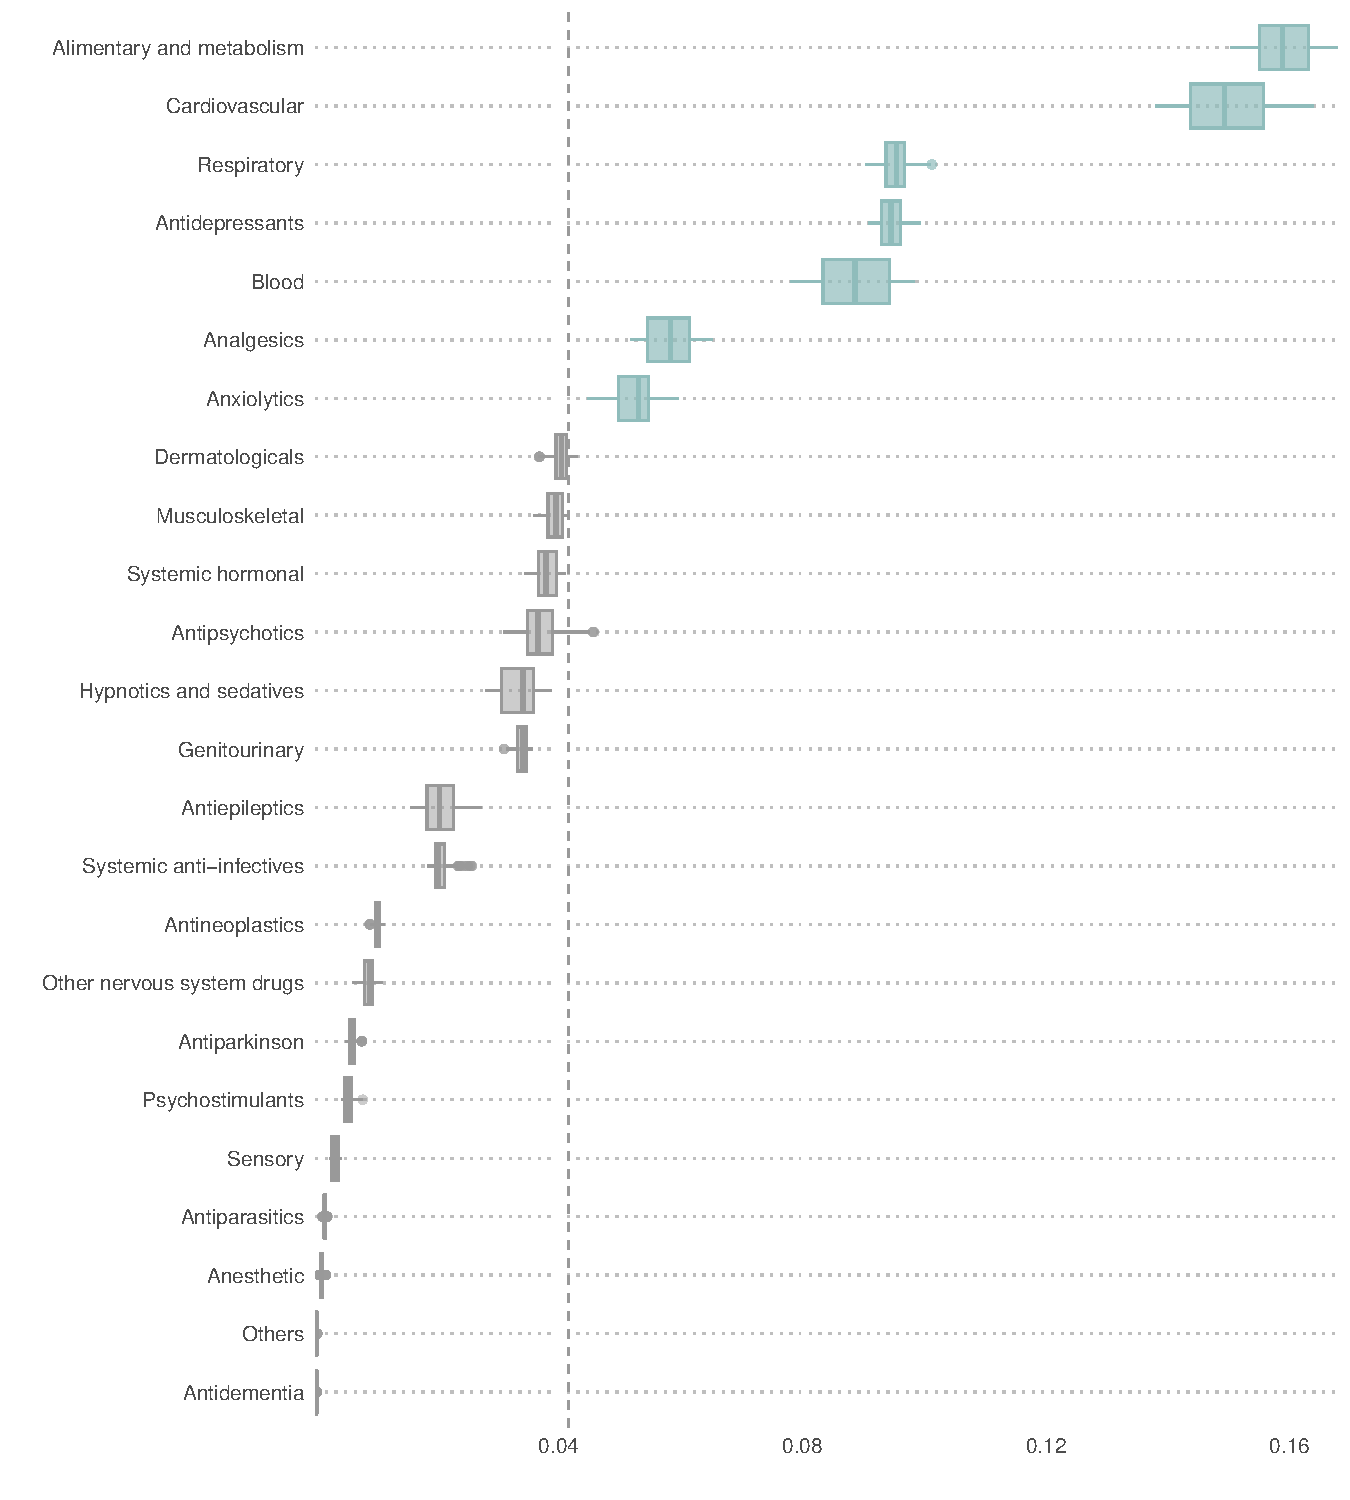
\includegraphics[width=1\linewidth,height=\textheight,keepaspectratio]{article_files/figure-pdf/fig-hi-eigen-1.pdf}

}

\caption{\label{fig-hi-eigen}Clusters of medication with a significant
co-prescription patterns on antidepressants and anxiolytics dispensing}

\end{figure}%

\section{Discussion}\label{discussion}

This network analysis of dispensing data in individuals using
antidepressants or anxiolytics revealed distinct co-prescription
patterns. While same-class co-prescription was more common among
antidepressant users, multi-class co-prescription predominated among
those receiving anxiolytics. Notably, in both groups, multi-class
co-prescription was at least ten times more prevalent than same-class
co-prescription. Seven medication classes exhibited high eigenvector
centrality, indicating their strong influence on co-prescription
dynamics. These include medications for the alimentary tract and
metabolism (ATC code \texttt{A}), blood and blood-forming organs
(\texttt{B}), cardiovascular system (\texttt{C}), respiratory system
(\texttt{R}), and analgesics (\texttt{N02}). These classes do not merely
appear frequently but also serve as key connectors within prescribing
networks, linking psychiatric treatments to chronic disease management.
Their centrality suggests that they play a role in structuring
multi-class co-prescription, either as standard co-prescriptions due to
clinical guidelines or as necessary adjuncts in managing comorbidities
or side effects, e.g., ATC \texttt{A} class. These findings align with
the theoretical basis of eigenvector centrality, which incorporates not
only the frequency of a node but also the influence of its connections.
Accordingly, medications with high dispensing volume may have lower
centrality if they are co-prescribed with less central or sparsely
connected drug classes.

The predomination of multi-class co-prescription among anxiolytics
recipients is consistent with the recommendations in the Dutch College
of General Practitioner (\emph{Nederlands Huisartsen Genootschap}/NHG)
\citep{NHG2019Anxiety}. Specifically, the NHG guideline for anxiety
disorders advises short-term benzodiazepine use, limited to two to four
weeks, as an adjunct to Selective Serotonin Reuptake Inhibitors (SSRIs)
during treatment initiation. In contrast, the NHG guideline for
depressive disorders recommends initiating pharmacotherapy with a single
SSRI and discourages the combination of multiple antidepressants
\citep{NHG2023Depression}. Therefore, the higher rate of multi-class
co-prescription observed among anxiolytic users is consistent with
evidence-based clinical practice, rather than an artifact of sampling or
measurement methods.

Our findings also align with previous research showing that
antidepressants and anxiolytics are frequently co-prescribed with other
medications \citep{Shrivastava2013}, and that multi-class regimens
contribute most to psychopharmaca polypharmacy
\citep{de2004polypharmacy}. Additionally, our study offers a more
granular view of these patterns by characterizing their network
properties. By distinguishing between same-class and multi-class
co-prescriptions and evaluating medication centrality, we discover that
certain drug classes function as hubs within the prescribing landscape.
These characteristics likely reflect the underlying burden of
multimorbidity in the population, where the bidirectional associations
between depression/anxiety and chronic illnesses is well established
\citep{qi2024longitudinal}. Conditions such as diabetes mellitus,
thyroid disorders, and asthma have been linked to an increased risk of
depression \citep{jang2024temporal}. The need for long-term
pharmacological management further drives co-prescription patterns.
Additionally, chronic illness-related anxiety can contribute to
heightened prescribing of anxiolytics \citep{lebel2020health}. This
underscores the interconnected nature of psychopharmaca prescribing
patterns and highlights the complexity of medication management in these
populations.

DPN complements traditional drug utilization analyses by capturing the
structural properties of prescribing behaviors. Beyond evaluating
individual drug utilization or basic pairwise co-prescriptions, DPN
provides a structural perspective by mapping the interconnections
between medications within a broader prescribing network
\citep{Bazzoni2015}. The network approach is a particularly useful
method for understanding complex prescribing dynamics, which allows for
the identification of central medication classes that influence
co-prescription patterns. The high centrality of certain medication
classes suggests they serve as critical connectors in treatment
regimens, providing the basis for further monitoring and evaluation.

By mapping the relationships between medications, DPN enables the
detection of patterns that would be challenging to observe through
standard statistical methods. For instance, the high centrality of
certain medication classes suggests that they play a pivotal role in
multi-class co-prescription, likely due to their involvement in managing
both psychiatric and non-psychiatric conditions. As such, network
analysis is a suitable approach for generating hypotheses for further
causal or predictive studies, which has also been thoroughly discussed
by \citet{Askar2021}.

We acknowledge several limitations in this study. First, data
aggregation at the population level resulted in the loss of
individual-level information, limiting interpretation to population
trends. Second, while the adjustment of weights based on DDD introduces
a novel element to the analysis, it is important to note that DDD values
are not always equal to one, as defined by the WHO ATC system. Our study
adopted a DDD-based weighting approach to refine network edges, aligning
with the recommendation of \citet{Cavallo2012}. The adjusted weighting
penalizes values deviating significantly from 1, reducing their impact
on the network. Future research should explore alternative weighting
techniques, such as patient-level dosage adjustments, to enhance network
precision.

Despite the limitations, our study demonstrates the utility of DPN as a
powerful, data-driven approach to analyzing medication dispensing data.
By modelling intricate co-prescription patterns, DPN filters medication
classes based on network properties, offering insights into prescribing
behaviors. These insights can reveal important trends in medication use,
which can be useful to pharmaceutical reviews and public health
monitoring. By capturing the complexity of drug prescription
relationships, DPN holds significant potential to improve
decision-making in both clinical and administrative contexts.

Future DPN studies on individuals using antidepressants or anxiolytics
should adopt a more fine-grained ATC classification to identify specific
medications driving co-prescription patterns within the currently
identified seven medication classes. A more granular approach could
reveal whether certain drugs disproportionately contribute to
multi-class co-prescription and whether these prescribing trends vary
across patient demographics or healthcare settings. Such insights could
refine our understanding of prescribing behaviors and inform targeted
interventions for optimizing medication regimens.

\section{Conclusion}\label{conclusion}

This study demonstrates the utility of DPN in uncovering the patterns of
co-prescriptions among antidepressants and anxiolytics recipients. We
found that multi-class regimens were markedly more prevalent,
particularly among anxiolytic users, consistent with clinical
guidelines. Moreover, we identified seven highly central medication
classes that act as hubs in the prescribing network, linking psychiatric
medications to the management of chronic somatic conditions. These
findings emphasize the role of multimorbidity in shaping co-prescription
behaviors and highlight the importance of these seven classes in both
psychiatric care and broader chronic disease management. Our study
contributes a network-based perspective to drug utilization research,
offering an alternative approach to identifying high-impact medication
classes that warrant further monitoring and future investigation.


\renewcommand\refname{References}
  \bibliography{ref.bib}



\end{document}
